\documentclass[a4paper,12pt,twoside]{memoir}

% Castellano
\usepackage[spanish,es-tabla]{babel}
\selectlanguage{spanish}
\usepackage[utf8]{inputenc}
\usepackage[T1]{fontenc}
\usepackage{lmodern} % scalable font
\usepackage{microtype}
\usepackage{placeins}

\RequirePackage{booktabs}
\RequirePackage[table]{xcolor}
\RequirePackage{xtab}
\RequirePackage{multirow}

% Links
\PassOptionsToPackage{hyphens}{url}\usepackage[colorlinks]{hyperref}
\hypersetup{
	allcolors = {red}
}

% Ecuaciones
\usepackage{amsmath}

% Rutas de fichero / paquete
\newcommand{\ruta}[1]{{\sffamily #1}}

% Párrafos
\nonzeroparskip

% Huérfanas y viudas
\widowpenalty100000
\clubpenalty100000

% Evitar solapes en el header
\nouppercaseheads

% Imagenes
\usepackage{graphicx}
\newcommand{\imagen}[2]{
	\begin{figure}[!h]
		\centering
		\includegraphics[width=0.9\textwidth]{#1}
		\caption{#2}\label{fig:#1}
	\end{figure}
	\FloatBarrier
}

\newcommand{\imagenflotante}[2]{
	\begin{figure}%[!h]
		\centering
		\includegraphics[width=0.9\textwidth]{#1}
		\caption{#2}\label{fig:#1}
	\end{figure}
}



% El comando \figura nos permite insertar figuras comodamente, y utilizando
% siempre el mismo formato. Los parametros son:
% 1 -> Porcentaje del ancho de página que ocupará la figura (de 0 a 1)
% 2 --> Fichero de la imagen
% 3 --> Texto a pie de imagen
% 4 --> Etiqueta (label) para referencias
% 5 --> Opciones que queramos pasarle al \includegraphics
% 6 --> Opciones de posicionamiento a pasarle a \begin{figure}
\newcommand{\figuraConPosicion}[6]{%
  \setlength{\anchoFloat}{#1\textwidth}%
  \addtolength{\anchoFloat}{-4\fboxsep}%
  \setlength{\anchoFigura}{\anchoFloat}%
  \begin{figure}[#6]
    \begin{center}%
      \Ovalbox{%
        \begin{minipage}{\anchoFloat}%
          \begin{center}%
            \includegraphics[width=\anchoFigura,#5]{#2}%
            \caption{#3}%
            \label{#4}%
          \end{center}%
        \end{minipage}
      }%
    \end{center}%
  \end{figure}%
}

%
% Comando para incluir imágenes en formato apaisado (sin marco).
\newcommand{\figuraApaisadaSinMarco}[5]{%
  \begin{figure}%
    \begin{center}%
    \includegraphics[angle=90,height=#1\textheight,#5]{#2}%
    \caption{#3}%
    \label{#4}%
    \end{center}%
  \end{figure}%
}
% Para las tablas
\newcommand{\otoprule}{\midrule [\heavyrulewidth]}
%
% Nuevo comando para tablas pequeñas (menos de una página).
\newcommand{\tablaSmall}[5]{%
 \begin{table}
  \begin{center}
   \rowcolors {2}{gray!35}{}
   \begin{tabular}{#2}
    \toprule
    #4
    \otoprule
    #5
    \bottomrule
   \end{tabular}
   \caption{#1}
   \label{tabla:#3}
  \end{center}
 \end{table}
}

%
%Para el float H de tablaSmallSinColores
\usepackage{float}

%
% Nuevo comando para tablas pequeñas (menos de una página).
\newcommand{\tablaSmallSinColores}[5]{%
 \begin{table}[H]
  \begin{center}
   \begin{tabular}{#2}
    \toprule
    #4
    \otoprule
    #5
    \bottomrule
   \end{tabular}
   \caption{#1}
   \label{tabla:#3}
  \end{center}
 \end{table}
}

\newcommand{\tablaApaisadaSmall}[5]{%
\begin{landscape}
  \begin{table}
   \begin{center}
    \rowcolors {2}{gray!35}{}
    \begin{tabular}{#2}
     \toprule
     #4
     \otoprule
     #5
     \bottomrule
    \end{tabular}
    \caption{#1}
    \label{tabla:#3}
   \end{center}
  \end{table}
\end{landscape}
}

%
% Nuevo comando para tablas grandes con cabecera y filas alternas coloreadas en gris.
\newcommand{\tabla}[6]{%
  \begin{center}
    \tablefirsthead{
      \toprule
      #5
      \otoprule
    }
    \tablehead{
      \multicolumn{#3}{l}{\small\sl continúa desde la página anterior}\\
      \toprule
      #5
      \otoprule
    }
    \tabletail{
      \hline
      \multicolumn{#3}{r}{\small\sl continúa en la página siguiente}\\
    }
    \tablelasttail{
      \hline
    }
    \bottomcaption{#1}
    \rowcolors {2}{gray!35}{}
    \begin{xtabular}{#2}
      #6
      \bottomrule
    \end{xtabular}
    \label{tabla:#4}
  \end{center}
}

%
% Nuevo comando para tablas grandes con cabecera.
\newcommand{\tablaSinColores}[6]{%
  \begin{center}
    \tablefirsthead{
      \toprule
      #5
      \otoprule
    }
    \tablehead{
      \multicolumn{#3}{l}{\small\sl continúa desde la página anterior}\\
      \toprule
      #5
      \otoprule
    }
    \tabletail{
      \hline
      \multicolumn{#3}{r}{\small\sl continúa en la página siguiente}\\
    }
    \tablelasttail{
      \hline
    }
    \bottomcaption{#1}
    \begin{xtabular}{#2}
      #6
      \bottomrule
    \end{xtabular}
    \label{tabla:#4}
  \end{center}
}

%
% Nuevo comando para tablas grandes sin cabecera.
\newcommand{\tablaSinCabecera}[5]{%
  \begin{center}
    \tablefirsthead{
      \toprule
    }
    \tablehead{
      \multicolumn{#3}{l}{\small\sl continúa desde la página anterior}\\
      \hline
    }
    \tabletail{
      \hline
      \multicolumn{#3}{r}{\small\sl continúa en la página siguiente}\\
    }
    \tablelasttail{
      \hline
    }
    \bottomcaption{#1}
  \begin{xtabular}{#2}
    #5
   \bottomrule
  \end{xtabular}
  \label{tabla:#4}
  \end{center}
}



\definecolor{cgoLight}{HTML}{EEEEEE}
\definecolor{cgoExtralight}{HTML}{FFFFFF}

%
% Nuevo comando para tablas grandes sin cabecera.
\newcommand{\tablaSinCabeceraConBandas}[5]{%
  \begin{center}
    \tablefirsthead{
      \toprule
    }
    \tablehead{
      \multicolumn{#3}{l}{\small\sl continúa desde la página anterior}\\
      \hline
    }
    \tabletail{
      \hline
      \multicolumn{#3}{r}{\small\sl continúa en la página siguiente}\\
    }
    \tablelasttail{
      \hline
    }
    \bottomcaption{#1}
    \rowcolors[]{1}{cgoExtralight}{cgoLight}

  \begin{xtabular}{#2}
    #5
   \bottomrule
  \end{xtabular}
  \label{tabla:#4}
  \end{center}
}




\graphicspath{ {./img/} }

% Capítulos
\chapterstyle{bianchi}
\newcommand{\capitulo}[2]{
	\setcounter{chapter}{#1}
	\setcounter{section}{0}
	\setcounter{figure}{0}
	\setcounter{table}{0}
	\chapter*{#2}
	\addcontentsline{toc}{chapter}{#2}
	\markboth{#2}{#2}
}

% Apéndices
\renewcommand{\appendixname}{Apéndice}
\renewcommand*\cftappendixname{\appendixname}

\newcommand{\apendice}[1]{
	%\renewcommand{\thechapter}{A}
	\chapter{#1}
}

\renewcommand*\cftappendixname{\appendixname\ }

% Formato de portada
\makeatletter
\usepackage{xcolor}
\newcommand{\tutor}[1]{\def\@tutor{#1}}
\newcommand{\course}[1]{\def\@course{#1}}
\newcommand{\tutorEmpresa}[1]{\def\@tutorEmpresa{#1}}
\definecolor{cpardoBox}{HTML}{E6E6FF}
\def\maketitle{
  \null
  \thispagestyle{empty}
  % Cabecera ----------------
\noindent
\includegraphics[width=\textwidth]{cabecera}\vspace{1cm}%
  \vfill
  % Título proyecto y escudo informática ----------------
  \colorbox{cpardoBox}{%
    \begin{minipage}{.8\textwidth}
      \vspace{.5cm}\Large
      \begin{center}
      \textbf{TFG del Grado en Ingeniería Informática}\vspace{.6cm}\\
      \textbf{\LARGE\@title{}}
      \end{center}
      \vspace{.2cm}
    \end{minipage}

  }%
  \hfill\begin{minipage}{.20\textwidth}
    
\includegraphics[width=\textwidth]{escudoInfor}
  \end{minipage}
  \vfill
  % Datos de alumno, curso y tutores ------------------
  \begin{center}%
  {%
    \noindent\LARGE
    Presentado por \@author{}\\ 
    en Universidad de Burgos --- \@date{}\\
    Tutor: \@tutor{}\\
    Tutor Empresa (Vicomtech): \@tutorEmpresa{}\\
  }%
  \end{center}%
  \null
  \cleardoublepage
  }
\makeatother


% Datos de portada
\title{Asistente para visitar museos mediante geolocalización de usuarios en entornos indoor \\Documentación Técnica}
\author{Mauricio José De Armas Garcia-Valdecasas}
\tutor{César Represa Pérez}
\tutorEmpresa{Mikel Zorrilla Berasategui}
\date{\today}

\begin{document}

\maketitle



\cleardoublepage



%%%%%%%%%%%%%%%%%%%%%%%%%%%%%%%%%%%%%%%%%%%%%%%%%%%%%%%%%%%%%%%%%%%%%%%%%%%%%%%%%%%%%%%%
\newpage\null\thispagestyle{empty}\newpage


%%%%%%%%%%%%%%%%%%%%%%%%%%%%%%%%%%%%%%%%%%%%%%%%%%%%%%%%%%%%%%%%%%%%%%%%%%%%%%%%%%%%%%%%



\noindent
\includegraphics[width=\textwidth]{cabecera}\vspace{1cm}

\noindent D. César Represa Pérez, profesor del departamento de Ingeniería Electromecánica, área de Tecnología Electrónica.

\noindent Expone:

\noindent Que el alumno D. Mauricio José De Armas Garcia-Valdecasas \nombre, con DNI 77555454Y, ha realizado el Trabajo Final de Grado en Ingeniería Informática titulado \textit{Asistente para visitar museos
mediante geolocalización de
usuarios en entornos indoor}. 

\noindent Y que dicho trabajo ha sido realizado por el alumno bajo la dirección del que suscribe, en virtud de lo cual se autoriza su presentación y defensa.

\begin{center} %\large
En Burgos, {\large \today}
\end{center}

\vfill\vfill\vfill

% Author and supervisor
\begin{minipage}{0.45\textwidth}
\begin{flushleft} %\large
Vº. Bº. del Tutor:\\[2cm]
D. César Represa Pérez
\end{flushleft}
\end{minipage}
\hfill
\begin{minipage}{0.45\textwidth}
\begin{flushleft} %\large
Vº. Bº. del co-tutor:\\[2cm]
Mikel Zorrilla Berasategui
\end{flushleft}
\end{minipage}
\hfill

\vfill

% para casos con solo un tutor comentar lo anterior
% y descomentar lo siguiente
%Vº. Bº. del Tutor:\\[2cm]
%D. nombre tutor


\frontmatter


\clearpage

% Indices
\tableofcontents

\clearpage

\listoffigures

\clearpage

\listoftables

\clearpage

\mainmatter

\appendix

\apendice{Plan de Proyecto Software}
\section{Introducción}
La fase de planificación de un proyecto es una de las fase clave cuando se quiere organizar el desarrollo de un proyecto. A grandes rasgos, se exponen las ideas a desarrollar teniendo en cuenta las limitaciones temporales y económicas que exigía el proyecto y la organización.

Este anexo será dividido en dos subapartados:
\begin{itemize}
  \item \textbf{Planificación temporal}: Especifica el formato y contenido de los planes para la gestión de un proyecto \textit{software}.
  \item \textbf{Estudio de viabilidad}: Permite hacer un estudio económico-legal para ver si el proyecto es viable o no. Este subapartado se divide en:
    \begin{itemize}
        \item \underline{Viabilidad económica}: Se hace una estimación de los costes de la aplicación.
        \item \underline{Viabilidad legal}: Se hace un análisis de las tecnologías en base a sus licencias y se tienen en cuenta las leyes actuales en relación al proyecto.
    \end{itemize}
\end{itemize}

\section{Planificación temporal}

Para la realización de este proyecto, la organización \textit{Vicomtech} propuso utilizar \textit{Scrum} como la metodología a utilizar para la realización del proyecto.

Esta metodología divide el trabajo en \textit{Sprints}, siendo la planificación de las tareas a realizar una de las fases mas importantes de esta metodología teniendo en cuenta la duración de cada \textit{sprint}, siendo normalmente de una semana.

\subsection{Sprint 0}

En este primer \textit{sprint} se expusieron, de manera general, todos los aspectos relevantes del proyecto, su arquitectura y cuáles iban a ser los puntos claves del proyecto para su desarrollo. Se investigaron soluciones similares, y posibles tecnologías en el desarrollo del proyecto. 

Este \textit{sprint} duró más de lo habitual, ya que al no conocer ningún aspecto relevante del proyecto y el desconocimiento de algunas de las tecnologías, se tuvo que hacer un gran trabajo de investigación.

\subsection{Sprint 1}

En este \textit{sprint} se decidió que se iba a comenzar por todos los conceptos relacionados con mapas, y sobre su aplicación sobre aplicaciones web en \textit{ReactJs}. Se hizo un trabajo de investigación sobre librerías de mapas para aplicaciones web y sus posibles adaptaciones para la localización \textit{indoor} de usuarios.

Este \textit{sprint} duró mas de lo planificado inicialmente, debido a que las librerías en \textit{Javascript} de mapas no tenían compatibilidad directa con \textit{ReactJs}. Por lo que finalmente se opto por adaptar la importación de la librería \textit{OpenLayers} y utilizar su código en \textit{Javascript vainilla} embebido en código \textit{React}.

\subsection{Sprint 2}

Este \textit{sprint} se basó en utilizar los planos del edificio de la empresa, geolocalizarlo en un \textit{software} llamado \textit{Qgis}, y exportarlo para poderlo utilizar como capa en la librería de mapas web \textit{OpenLayers}.

\subsection{Sprint 3}

En este \textit{sprint} el objetivo se basó en diseñar la \textit{API} que conectaría con la base de datos en archivo \textit{YAML}, para poder generar una versión inicial, en lenguaje \textit{Python} y desplegado en \textit{Docker}, a completar para desarrollar la funcionalidad. Además se implementó un \textit{ORM} de la librería \textit{SQLAlchemy}, para poder interactuar con el contenedor \textit{docker} de la base de datos de manera dinámica en código \textit{Python}.

En cuestiones de funcionalidad, se implementaron parcialmente las funcionalidades de distintos \textit{endpoints}. Pero se dejaron algunas tareas para el siguiente \textit{sprint}.
\begin{figure}[H]
    \centering
    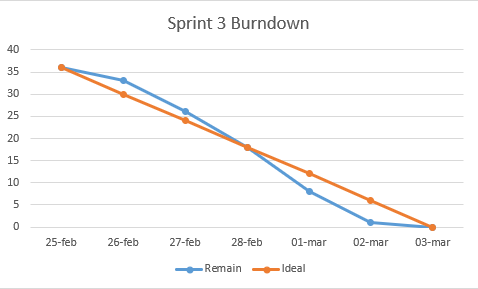
\includegraphics[width=10cm,height=10cm,keepaspectratio]{img/Sprint3_burndow.png}
    \caption{Sprint 3 Burndown.}
    \label{fig:sprint3_burndown}
\end{figure}
\subsection{Sprint 4}

En este sprint el objetivo fue terminar las funcionalidades de los distintos \textit{endpoints} no implementados en el \textit{sprint} anterior, e investigar acerca de las distintas soluciones de \textit{geofencing} existentes para implementar en el proyecto, se eligió \textit{Tile38} como librería \textit{geofencing}.
\begin{figure}[H]
    \centering
    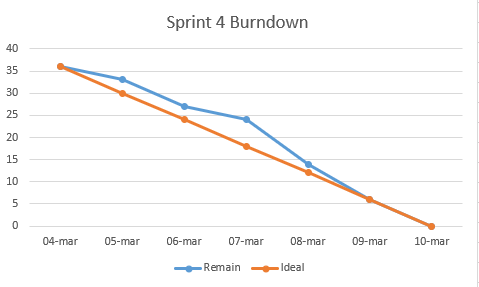
\includegraphics[width=10cm,height=10cm,keepaspectratio]{img/Sprint4_burndow.png}
    \caption{Sprint 4 Burndown.}
    \label{fig:sprint4_burndown}
\end{figure}
\subsection{Sprint 5}

En este Sprint se implementó la librería de los \textit{pyle38} para interactuar con los \textit{dockers} de \textit{Tile38} en la \textit{API} y se trabajó en el \textit{frontend} de la aplicación.
\begin{figure}[H]
    \centering
    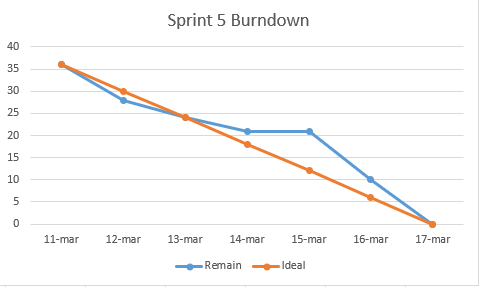
\includegraphics[width=10cm,height=10cm,keepaspectratio]{img/Sprint5_burndow.png}
    \caption{Sprint 5 Burndown.}
    \label{fig:sprint5_burndown}
\end{figure}
\subsection{Sprint 6}
En este \textit{sprint} el objetivo fue trabajar en el \textit{frontend} de la aplicación para poder tener una versión de producción con un buena interfaz de usuario, que genere una buena experiencia de usuario y que no cause confusiones al usuario al utilizar la parte del mapa con otras partes de la aplicación.
\begin{figure}[H]
    \centering
    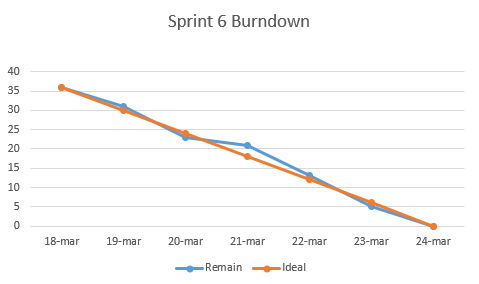
\includegraphics[width=10cm,height=10cm,keepaspectratio]{img/Sprint6_burndow.png}
    \caption{Sprint 6 Burndown.}
    \label{fig:sprint6_burndown}
\end{figure}
\subsection{Sprint 7}
En este \textit{sprint} el objetivo fue documentar toda la aplicación de manera profunda, y ayudar con otras partes del desarrollo a compañeros, así como pulir mis partes de la aplicación y testearla manualmente para su correcto funcionamiento en distintos contextos.

\subsection{Resumen}
En la tabla-resumen se muestran los tiempos dedicados a cada una de las distintas tareas:

\begin{table}[H]
    \setlength{\tabcolsep}{20pt}
    \centering
    \begin{tabular}{@{}l r}
    \noalign{\hrule height 0.8pt}  Categoria &  Tiempo(horas)\\\hline
      Investigación &  47\\
      Desarrollo &  252\\
      Arreglo de errores &  15\\
      Documentación &  70\\
    \hline Total: & 384\\
    \noalign{\hrule height 0.8pt}
    \end{tabular}
    \caption{Tabla recuento de horas de trabajo.}
    \label{tab:Table-counting-working-hours}
\end{table}


\begin{figure}[H]
    \centering
    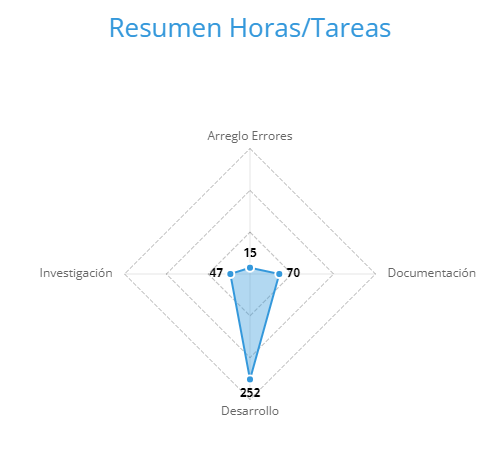
\includegraphics[width=10cm,height=10cm,keepaspectratio]{img/Resumen Horas_Tareas_ (1).png}
    \caption{Gráfico-Resumen horas dedicadas al proyecto.}
    \label{fig:graph-time-working}
\end{figure}
\section{Estudio de viabilidad}
En este punto se hará un análisis desde el punto de vista económica y legal para la viabilidad del proyecto. 
\subsection{Viabilidad económica}
Para la viabilidad económica, se procederán a desglosar los costes que tendrá el desarrollo de la aplicación.

Primero debemos de nombrar los costes del personal que desarrollara la aplicación. Siendo un solo empleado el que realiza la aplicación durante cinco meses el desglose sería:
\FloatBarrier
\begin{table}[h]
    \setlength{\tabcolsep}{20pt}
    \centering
    \begin{tabular}{@{}l r}
    \noalign{\hrule height 0.8pt}  Concepto &  Coste en euros\\\hline
      Salario neto mensual &  1221,75\\
      IRPF(17\%) &  255\\
      Seguridad Social(23,60\%) &  384,44\\
      Salario mensual bruto &  1500\\
    \hline Total 5 meses: & 7500\\
    \noalign{\hrule height 0.8pt}
    \end{tabular}
    \caption{Tabla de coste de personal.}
    \label{tab:table-crew-costs}
\end{table}
\FloatBarrier
Con esto se tendría que hacer un gaste para componentes hardware, quedando otro desglose de:
\FloatBarrier
\begin{table}[h]
    \setlength{\tabcolsep}{20pt}
    \centering
    \begin{tabular}{@{}l r}
    \noalign{\hrule height 0.8pt}  Concepto &  Coste en euros\\\hline
      \textit{MDEK1001 Kit} de desarrollo (12 unidades) &  2456,28\\
      \textit{Rasperry Pi 3} (2 unidades)&  63\\

    \hline Total: & 2519,28\\
    \noalign{\hrule height 0.8pt}
    \end{tabular}
    \caption{Tabla de coste de hardware.}
    \label{tab:table-hardware-costs}
\end{table}
\FloatBarrier
Quedando así la suma de costes totales de la aplicación en:
\FloatBarrier
\begin{table}[h]
    \setlength{\tabcolsep}{20pt}
    \centering
    \begin{tabular}{@{}l r}
    \noalign{\hrule height 0.8pt}  Concepto &  Coste en euros\\\hline
      Personal &  7500\\
      Hardware &  2519,28\\
    \hline Total: & 10019,28\\
    \noalign{\hrule height 0.8pt}
    \end{tabular}
    \caption{Tabla de costes totales.}
    \label{tab:table-total-costs}
\end{table}
\FloatBarrier
Teniendo así que hacer una explotación comercial del \textit{software} para poder recuperar la inversión que se ha hecho en el desarrollo de la aplicación.

\subsection{Viabilidad legal}

Para la explotación comercial del \textit{software} primero se tienen que revisar las licencias legales de las herramientas y librerías utilizadas para el desarrollo de la aplicación.

En esta lista están todas las librerías y herramientas necesarias para la ejecución de la aplicación junto con su correspondiente tipo de licencia:


\FloatBarrier
\begin{table}[h]
    \setlength{\tabcolsep}{5pt}
    \centering
    \begin{tabular}{l p{3cm} p{5cm} p{3cm}}
    Dependencia &  Versión & Descripción & Licencia\\\hline
      Javascript &  ECMAScript 2018 & Lenguaje base de la webapp & CC Atributtion\\
      ReactJS &  17.0 & Framework & MIT\\
      Python &  3.7.0 & Lenguaje API & Python\\
      Flask &  2.0 & Framework API & BSD\\
      SqlAlchemy &  1.4.37 & Librería ORM para conexión con Base de datos & MIT\\
      OpenLayers &  6.14.1 & Librería de Mapas & BSD\\
      JanusWebRTC &  1.0.2 & Librería de \textit{Streaming} de audio y vídeo & GNU\\
    \hline
    \noalign{\hrule height 0.8pt}
    \end{tabular}
    \caption{Tabla dependencias-licencias.}
    \label{tab:table-dependencies-licenses}
\end{table}
\FloatBarrier

Una vez expuestas las licencias de las librerías, la que mas se adapta a nuestro proyecto es \textit{GPLv3} proporcionando derechos de libre uso, de estudio y compartición en copia y la modificación del \textit{software}, informando de los cambios realizados estando bajo la misma licencia.
\apendice{Especificación de Requisitos}
En este apartado se procederá a explicar el diseño de requisitos necesario para el desarrollo de este proyecto.

\section{Introducción}
En este apéndice se van a describir los requisitos que definen como el comportamiento con el que se va a construir el sistema del proyecto.
\section{Objetivos generales}
Los objetivos generales del proyecto van a ser:
\begin{itemize}
    \item Desarrollar una \textit{API} funcional conectada a una base de datos dando servicio para gestionar instancias de tipo: 
        \begin{itemize}
            \item \textit{\textbf{Rooms.}}
            \item \textit{\textbf{Tags.}}
            \item \textit{\textbf{Anchors.}}
            \item \textit{\textbf{Users.}}
            \item \textit{\textbf{Artworks.}}
            
        \end{itemize}   
    \item Desarrollar una aplicación web que contenga un mapa mostrando:
        \begin{itemize}
            \item \textbf{\textit{Rooms} dibujadas por los usuarios guía.}
            \item \textbf{\textit{Tags} con su localización \textit{indoor} a tiempo real.}
            \item \textbf{\textit{Anchors} con su localización \textit{indoor} real en el mapa.}
        \end{itemize} 
    \item Dar acceso a la aplicación por tipo de usuario y por distintas restricciones de sesiones diseñadas.
\end{itemize}
\section{Catálogo de requisitos}
\subsection{Requisitos Funcionales}
\begin{itemize}
    \item \textbf{RF 1 - Gestión de usuarios}. La aplicación debe ser capaz de gestionar las sesiones de los usuarios.
        \begin{itemize}
            \item \textbf{RF 1.1 - Creación de la sesión}. El usuario debe ser capaz de hacer \textit{Login} si el alias introducido no existe en la base de datos.
            \item \textbf{RF 1.2 - Reutilización de la sesión}. El usuario debe ser capaz de hacer \textit{Login} si el alias existe en la base de datos y no está enlazado con ninguna \textit{Tag}.
            \item \textbf{RF 1.3 - Enlace con un \textit{Tag}}. Un usuario debe ser capaz de enlazarse con un \textit{Tag} sino esta enlazado a otro usuario.
        \end{itemize}
    \item \textbf{RF 2 - Gestión de \textit{Tags}}. La aplicación debe ser capaz de gestionar las \textit{Tags}.
        \begin{itemize}
            \item \textbf{RF 2.1 - Creación de \textit{Tag}}. Las \textit{Raspberries} deben ser capaces de crear \textit{Tags}.
            \item \textbf{RF 2.2 - Modificación de datos de un \textit{Tag}}. Las \textit{Raspberries} deben ser capaces de modificar los datos de las \textit{Tags}.
            \item \textbf{RF 2.3 - Eliminación de un \textit{Tag}}. Las \textit{Raspberries} deben ser capaces de eliminar un \textit{Tag}.
            \item \textbf{RF 2.4 - Lectura de un \textit{Tag}}. La aplicación debe ser capaz de leer un determinado \textit{Tag}.
        \end{itemize}
    \item \textbf{RF 3 - Gestión de \textit{Anchors}}. La aplicación debe ser capaz de gestionar las \textit{Anchors}.
        \begin{itemize}
            \item \textbf{RF 3.1 - Creación de \textit{Anchor}}.  Las \textit{Raspberries} deben ser capaces de crear un \textit{Anchor}.
            \item \textbf{RF 3.2 - Modificación de datos de un \textit{Anchor}}. Las \textit{Raspberries} o los usuarios deben ser capaces de modificar datos en los \textit{Anchors}.
            \item \textbf{RF 3.4 - Eliminación de un \textit{Anchor}}. Las \textit{Raspberries} deben ser capaces de eliminar un \textit{Anchor}.
            \item \textbf{RF 3.5 - Lectura de un \textit{Anchor}}. La aplicación debe ser capaz de leer un \textit{Anchor}.
        \end{itemize}
    \item \textbf{RF 4 - Gestión de \textit{Rooms}}. La aplicación debe ser capaz de gestionar las \textit{Rooms}.
        \begin{itemize}
            \item \textbf{RF 4.1 - Creación de una \textit{Room}}. Un guía debe ser capaz de crear una \textit{Room}.
            \item \textbf{RF 4.2 - Eliminación de una \textit{Room}}. Un guía debe ser capaz de eliminar una \textit{Room}.
            \item \textbf{RF 4.3 - Lectura de una \textit{Room}}. La aplicación debe ser capaz de leer una \textit{Room}.
        \end{itemize}
    
    \item \textbf{RF 5 - \textit{Geofencing}}. La aplicación debe ser capaz de gestionar el \textit{geofencing} de \textit{Tags} y \textit{Rooms}.
        \begin{itemize}
            \item \textbf{RF 5.1 - Saber en que \textit{Room} esta un usuario determinado}. La aplicación debe ser capaz de determinar en que \textit{Room} está un usuario.
            \item \textbf{RF 5.2 - Saber cuantos usuarios están en una \textit{Room}}. la aplicación debe ser capaz de saber cuantos usuarios para hay en una \textit{Room}.
        \end{itemize}


    
\end{itemize}
\subsection{Requisitos No Funcionales}
\begin{itemize}
    \item \textbf{RNF1 - Tiempo de respuesta}: La aplicación debe ser capaz de tener tiempos de respuesta razonables de cara al usuario.
    \item \textbf{RNF2 - Usabilidad}: La aplicación debe de ser intuitiva teniendo una buena interfaz de usuario en su uso para proporcionar una buena experiencia de usuario.
    \item \textbf{RNF3 - Seguridad}: La aplicación ha de tener un mínimo de medidas de seguridad, siendo un proyecto de investigación pero posible producto.
    \item \textbf{RNF4 - Documentación}: La aplicación ha de tener una documentación de calidad que tenga toda la información necesaria para el entendimiento del proyecto, y el código debidamente comentado.
    
\end{itemize}
\section{Especificación de requisitos}
\subsection{Actores}
\begin{itemize}
    \item \textbf{Usuario}: Se considera como actor a un usuario, siendo este el que está o va a estar enlazado a una \textit{Tag} y recibe una visita.
    \item \textbf{Guía}: Se considera como guía al usuario que tiene permiso para entrar a distintas paginas de la aplicación web interactuando con ellas y da visitas. 
    \item \textit{\textbf{Raspberry}}: Se ha considerado la entidad \textit{Raspberry} como actor, debido a que interactúa de manera activa en los requisitos funcionales de manera que pueda cambiar la información de Tags cada segundo.
\end{itemize}
\subsection{Casos de uso}

Esquema general de los casos de uso:
\FloatBarrier
\begin{figure}[h]
    \centering
    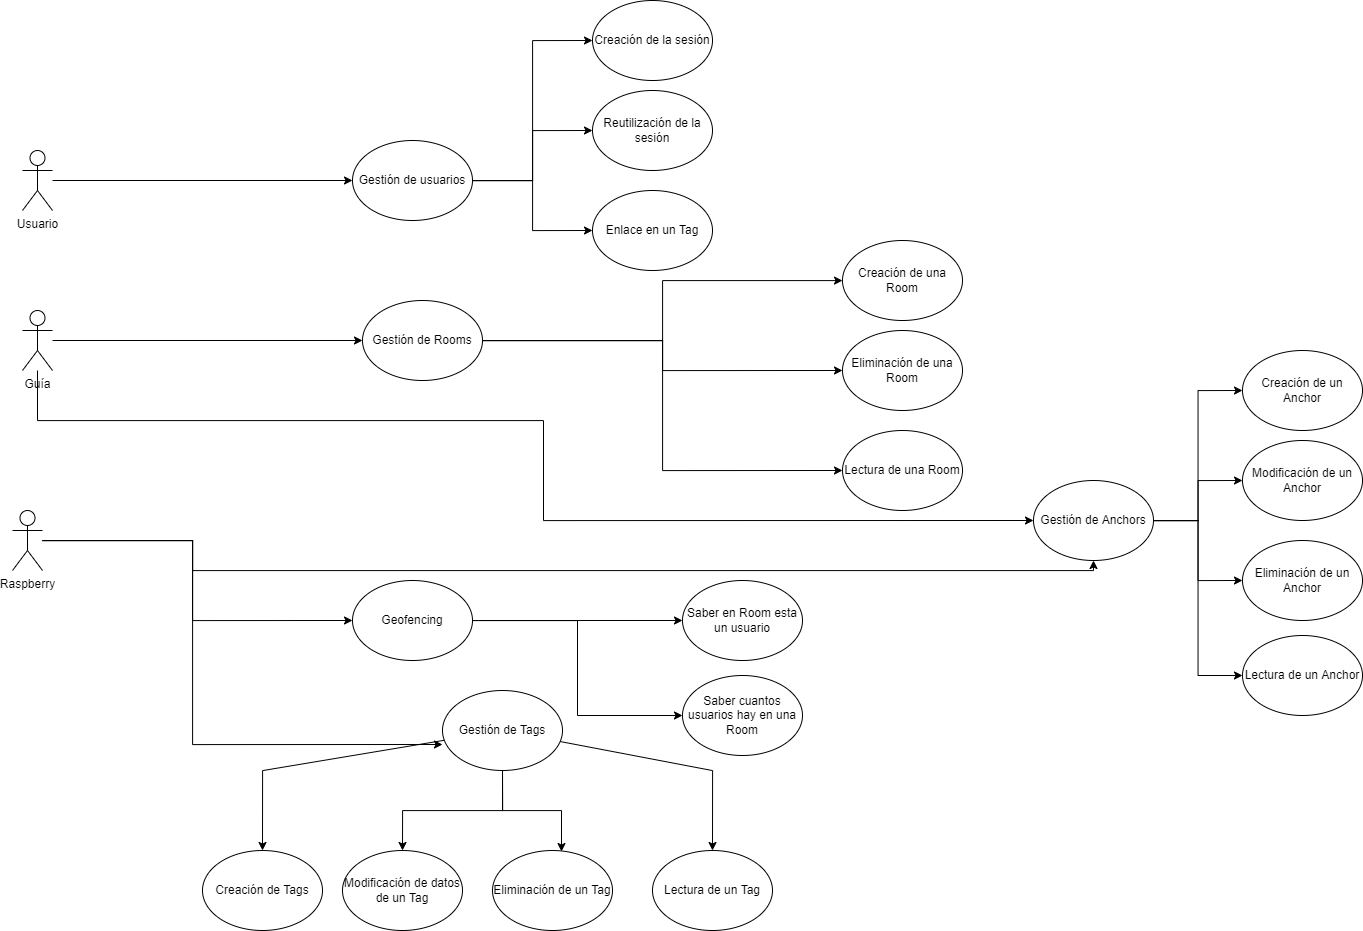
\includegraphics[width=15cm,height=15cm,keepaspectratio]{img/Diagrama General de Casos de uso.drawio (1).png}
    \caption{Diagrama General de Casos de uso.}
    \label{fig:diagrama_general_de_casos_de_uso}
\end{figure}
\FloatBarrier

\begin{table}[H]
    \centering
    \begin{tabular}{p{0.2\textwidth}CGC}
        \hline

        \multicolumn{4}{l}{Caso de uso 1: Gestión de usuarios}\\\hline
        \multirow{2}{*}{Descripción}&\multicolumn{3}{l}{La aplicación debe ser capaz de gestionar
        las sesiones}\\
        &\multicolumn{3}{l}{ de los usuarios.}\\\hline
        \multirow{4}{*}{Requisitos}&\multicolumn{3}{l}{RF 1.1}\\
        \cline{2-4}
        &\multicolumn{3}{l}{RF 1.2}\\
        \cline{2-4}
        &\multicolumn{3}{l}{RF 1.3}\\
        \cline{2-4}
        &\multicolumn{3}{l}{RF 2.4}\\\hline
        
        \multicolumn{1}{l}{Precondiciones}&\multicolumn{3}{l}{La \textit{API} tenga conexión activa con la \textit{bbdd}.}\\\hline
        \multirow{3}{*}{Flujo normal}&\multicolumn{1}{l}{Paso}&\multicolumn{2}{l}{Acción}\\
        \cline{2-4}
        &\multicolumn{1}{l}{1}&\multicolumn{2}{l}{El usuario ejecuta la \textit{WebApp}.}\\
        \cline{2-4}
        &\multicolumn{1}{l}{2}&\multicolumn{2}{l}{El usuario interacciona con el formulario de \textit{Login}.}\\
        \hline
        \multicolumn{1}{l}{Postcondiciones}&\multicolumn{3}{l}{}\\\hline
        \multicolumn{1}{l}{Excepciones}&\multicolumn{3}{l}{Error de \textit{CORS}.}\\\hline
        \multicolumn{1}{l}{Importancia}&\multicolumn{3}{l}{Alta.}\\\hline
        \multicolumn{1}{l}{Urgencia}&\multicolumn{3}{l}{Alta.}\\\hline
        \multicolumn{1}{l}{Comentarios}&\multicolumn{3}{l}{}\\\hline

    \end{tabular}
    \caption{Caso de uso 1: Gestión de usuarios.}
    \label{tab:Caso de uso 1: Gestión de usuarios}
\end{table}

\begin{table}[H]
    \centering
    \begin{tabular}{p{0.2\textwidth}CGC}
        \hline

        \multicolumn{4}{l}{Caso de uso 2: Creación de la sesión}\\\hline
        \multirow{2}{*}{Descripción}&\multicolumn{3}{l}{El usuario debe poder crear una nueva
        sesión con un}\\
        &\multicolumn{3}{l}{alias específico.}\\\hline
        \multirow{3}{*}{Requisitos}&\multicolumn{3}{l}{RF 1.1}\\
        \cline{2-4}
        &\multicolumn{3}{l}{RF 1.3}\\
        \cline{2-4}
        &\multicolumn{3}{l}{RF 2.4}\\
        \hline
        
        \multicolumn{1}{l}{Precondiciones}&\multicolumn{3}{l}{Conexión con la \textit{bbdd}.}\\\hline
        \multirow{6}{*}{Flujo normal}&\multicolumn{1}{l}{Paso}&\multicolumn{2}{l}{Acción}\\
        \cline{2-4}
        &\multicolumn{1}{l}{1}&\multicolumn{2}{l}{El usuario abre la pagina web.}\\
        \cline{2-4}
        &\multicolumn{1}{l}{2}&\multicolumn{2}{l}{Se comprueba que el usuario no existe.}\\
        \cline{2-4}
        &\multicolumn{1}{l}{3}&\multicolumn{2}{l}{Se comprueba que la tag no está enlazada a ningún usuario.}\\
        \cline{2-4}
        &\multicolumn{1}{l}{4}&\multicolumn{2}{l}{Se crea el usuario en la \textit{bbdd}.}\\
        \cline{2-4}
        &\multicolumn{1}{l}{5}&\multicolumn{2}{l}{Se enlaza la \textit{Tag} al usuario.}\\\hline
        \multicolumn{1}{l}{Postcondiciones}&\multicolumn{3}{l}{Se accede al chat.}\\\hline
        \multicolumn{1}{l}{Excepciones}&\multicolumn{3}{l}{Error de \textit{CORS}.}\\\hline
        \multicolumn{1}{l}{Importancia}&\multicolumn{3}{l}{Alta.}\\\hline
        \multicolumn{1}{l}{Urgencia}&\multicolumn{3}{l}{Alta.}\\\hline
        \multicolumn{1}{l}{Comentarios}&\multicolumn{3}{l}{}\\\hline

    \end{tabular}
    \caption{Caso de uso 2: Creación de la sesión.}
    \label{tab:Caso de uso 2: Creación de la sesión}
\end{table}

\begin{table}[H]
    \centering
    \begin{tabular}{p{0.2\textwidth}lGC}
        \hline
        \multicolumn{4}{l}{Caso de uso 3: Reutilización de la sesión}\\\hline
        \multirow{3}{*}{Descripción}&\multicolumn{3}{l}{El usuario debe ser capaz
        de hacer \textit{Login}}\\
        &\multicolumn{3}{l}{si el alias existe en la base de datos}\\
        &\multicolumn{3}{l}{y no está
        enlazado con ninguna \textit{Tag}.}\\\hline
        
        \multirow{3}{*}{Requisitos}&\multicolumn{3}{l}{RF 1.2}\\
        \cline{2-4}
        &\multicolumn{3}{l}{RF 1.3}\\
        \cline{2-4}
        &\multicolumn{3}{l}{RF 2.4}\\
        \hline
        
        \multicolumn{1}{l}{Precondiciones}&\multicolumn{3}{l}{Conexión con la \textit{bbdd}.}\\\hline
        \multirow{5}{*}{Flujo normal}&\multicolumn{1}{l}{Paso}&\multicolumn{2}{l}{Acción}\\
        \cline{2-4}
        &\multicolumn{1}{l}{1}&\multicolumn{2}{l}{El usuario abre la pagina web.}\\
        \cline{2-4}
        &\multicolumn{1}{l}{2}&\multicolumn{2}{l}{Se comprueba que el usuario existe.}\\
        \cline{2-4}
        &\multirow{2}{*}{4}&\multicolumn{2}{l}{Se comprueba que el usuario existe o no}\\
                           &&\multicolumn{2}{l}{existe, sin estar usado.}\\
        \cline{2-4}
        \cline{2-4}
        &\multicolumn{1}{l}{5}&\multicolumn{2}{l}{Se enlaza la \textit{Tag} al usuario.}\\\hline
        \multicolumn{1}{l}{Postcondiciones}&\multicolumn{3}{l}{Se accede a la página chat.}\\\hline
        \multicolumn{1}{l}{Excepciones}&\multicolumn{3}{l}{Error de \textit{CORS}.}\\\hline
        \multicolumn{1}{l}{Importancia}&\multicolumn{3}{l}{Alta.}\\\hline
        \multicolumn{1}{l}{Urgencia}&\multicolumn{3}{l}{Alta.}\\\hline
        \multicolumn{1}{l}{Comentarios}&\multicolumn{3}{l}{}\\\hline

    \end{tabular}
    \caption{Caso de uso 3: Reutilización de la sesión.}
    \label{tab:Caso de uso 3: Reutilización de la sesión}
\end{table}

\begin{table}[H]
    \centering
    \begin{tabular}{ClCC}
        \hline

        \multicolumn{4}{l}{Caso de uso 4: Enlace con un \textit{Tag}}\\\hline
    
        \multirow{2}{*}{Descripción}&\multicolumn{3}{l}{Un usuario debe ser capaz de
        enlazarse con un \textit{Tag}}\\
        &\multicolumn{3}{l}{sino esta enlazado a otro usuario.}\\\hline
        \multirow{1}{*}{Requisitos}&\multicolumn{3}{l}{RF 1.3}\\
        \hline
        
        \multicolumn{1}{l}{Precondiciones}&\multicolumn{3}{l}{Conexión con la \textit{bbdd}.}\\\hline
       
        \multirow{5}{*}{Flujo normal}&\multicolumn{1}{l}{Paso}&\multicolumn{2}{l}{Acción}\\
        \cline{2-4}
        &\multicolumn{1}{l}{1}&\multicolumn{2}{l}{El usuario abre la pagina web.}\\
        \cline{2-4}
        &\multirow{2}{*}{4}&\multicolumn{2}{l}{Se comprueba que el usuario existe o no}\\
                           &&\multicolumn{2}{l}{existe, sin estar usado.}\\
        \cline{2-4}
        &\multirow{2}{*}{3}&\multicolumn{2}{l}{Se comprueba que la \textit{Tag} no está enlazada}\\
                           &&\multicolumn{2}{l}{a ningún usuario.}\\
        \cline{2-4}
        &\multicolumn{1}{l}{5}&\multicolumn{2}{l}{Se enlaza la \textit{Tag} al usuario.}\\\hline
        \multicolumn{1}{l}{Postcondiciones}&\multicolumn{3}{l}{Se enlaza el usuario a la \textit{Tag}.}\\\hline
        \multicolumn{1}{l}{Excepciones}&\multicolumn{3}{l}{Error \textit{CORS}.}\\\hline
        \multicolumn{1}{l}{Importancia}&\multicolumn{3}{l}{Alta.}\\\hline
        \multicolumn{1}{l}{Urgencia}&\multicolumn{3}{l}{Alta.}\\\hline
        \multicolumn{1}{l}{Comentarios}&\multicolumn{3}{l}{}\\\hline

    \end{tabular}
    \caption{Caso de uso 4: Enlace con un \textit{Tag}.}
    \label{tab:Caso de uso 4: Enlace con un Tag}
\end{table}

\begin{table}[H]
    \centering
    \begin{tabular}{p{0.2\textwidth}CGC}
        \hline

        \multicolumn{4}{l}{Caso de uso 5: Gestión de \textit{Tags}}\\\hline
        \multicolumn{1}{l}{Descripción}&\multicolumn{3}{l}{La aplicación debe ser capaz de gestionar
las \textit{Tags}.}\\\hline
        \multirow{4}{*}{Requisitos}&\multicolumn{3}{l}{RF 2.1}\\
        \cline{2-4}
        &\multicolumn{3}{l}{RF 2.2}\\
        \cline{2-4}
        &\multicolumn{3}{l}{RF 2.3}\\
        \cline{2-4}
        &\multicolumn{3}{l}{RF 2.4}\\\hline
        
        \multicolumn{1}{l}{Precondiciones}&\multicolumn{3}{l}{Conexión con la base de datos.}\\\hline
        \multirow{3}{*}{Flujo normal}&\multicolumn{1}{l}{Paso}&\multicolumn{2}{l}{Acción}\\
        \cline{2-4}
        &\multicolumn{1}{l}{1}&\multicolumn{2}{l}{Inicializa el sistema de geolocalización.}\\
        \cline{2-4}
        &\multicolumn{1}{l}{2}&\multicolumn{2}{l}{Se comprueba si la \textit{Tag} existe, sino se añade.}\\\hline

        \multicolumn{1}{l}{Postcondiciones}&\multicolumn{3}{l}{}\\\hline
        \multicolumn{1}{l}{Excepciones}&\multicolumn{3}{l}{Error de conexión de la \textit{bbdd}.}\\\hline
        \multicolumn{1}{l}{Importancia}&\multicolumn{3}{l}{Alta.}\\\hline
        \multicolumn{1}{l}{Urgencia}&\multicolumn{3}{l}{Alta.}\\\hline
        \multicolumn{1}{l}{Comentarios}&\multicolumn{3}{l}{}\\\hline

    \end{tabular}
    \caption{Caso de uso 5: Gestión de \textit{Tags}.}
    \label{tab:Caso de uso 5: Gestión de Tags}
\end{table}

\begin{table}[H]
    \centering
    \begin{tabular}{p{0.2\textwidth}CGC}
        \hline

        \multicolumn{4}{l}{Caso de uso 6: Creación de \textit{Tag}}\\\hline
        \multicolumn{1}{l}{Descripción}&\multicolumn{3}{l}{Las Raspberries deben ser capaces
de crear \textit{Tags}.}\\\hline
        \multirow{1}{*}{Requisitos}&\multicolumn{3}{l}{RF 2.1}\\\hline
        
        \multicolumn{1}{l}{Precondiciones}&\multicolumn{3}{l}{Conexión con la \textit{bbdd}.}\\\hline
        \multirow{4}{*}{Flujo normal}&\multicolumn{1}{l}{Paso}&\multicolumn{2}{l}{Acción}\\
        \cline{2-4}
        &\multicolumn{1}{l}{1}&\multicolumn{2}{l}{Inicializa el sistema de geolocalización.}\\
        \cline{2-4}
        &\multicolumn{1}{l}{2}&\multicolumn{2}{l}{Se comprueba si la \textit{Tag} existe.}\\
        \cline{2-4}
        &\multicolumn{1}{l}{2}&\multicolumn{2}{l}{Si no existe se añade la \textit{Tag}.}\\\hline
        \multicolumn{1}{l}{Postcondiciones}&\multicolumn{3}{l}{Se actualiza la base de datos.}\\\hline
        \multicolumn{1}{l}{Excepciones}&\multicolumn{3}{l}{Error con la \textit{bbdd}.}\\\hline
        \multicolumn{1}{l}{Importancia}&\multicolumn{3}{l}{Alta}\\\hline
        \multicolumn{1}{l}{Urgencia}&\multicolumn{3}{l}{Alta.}\\\hline
        \multicolumn{1}{l}{Comentarios}&\multicolumn{3}{l}{}\\\hline

    \end{tabular}
    \caption{Caso de uso 6: Creación de \textit{Tag}.}
    \label{tab:Caso de uso 6: Creación de Tag}
\end{table}

\begin{table}[H]
    \centering
    \begin{tabular}{p{0.2\textwidth}CGC}
        \hline

        \multicolumn{4}{l}{Caso de uso 7: Modificación de datos de \textit{Tag}}\\\hline
        \multirow{2}{*}{Descripción}&\multicolumn{3}{l}{Las \textit{Raspberries}
        deben ser capaces }\\
        &\multicolumn{3}{l}{de modificar los datos de las \textit{Tags}.}\\\hline
        \multirow{1}{*}{Requisitos}&\multicolumn{3}{l}{RF 2.2 }\\\hline
        \multirow{1}{*}{Precondiciones}&\multicolumn{3}{l}{Conexión con la base de datos.}\\\hline
        
        \multirow{6}{*}{Flujo normal}&\multicolumn{1}{l}{Paso}&\multicolumn{2}{l}{Acción}\\
        \cline{2-4}
        &\multicolumn{1}{l}{1}&\multicolumn{2}{l}{Inicializa el sistema de geolocalización.}\\
        \cline{2-4}
        &\multicolumn{1}{l}{2}&\multicolumn{2}{l}{Se comprueba si la \textit{Tag} existe.}\\
        \cline{2-4}
        &\multicolumn{1}{l}{2}&\multicolumn{2}{l}{Si no existe se añade la \textit{Tag}.}\\
        \cline{2-4}
        &\multicolumn{1}{l}{2}&\multicolumn{2}{l}{Se modifican datos de la \textit{Tag}.}\\\hline
        \multicolumn{1}{l}{Postcondiciones}&\multicolumn{3}{l}{Se actualiza la base de datos.}\\\hline
        \multicolumn{1}{l}{Excepciones}&\multicolumn{3}{l}{Error con la conexión de la \textit{bbdd}.}\\\hline
        \multicolumn{1}{l}{Importancia}&\multicolumn{3}{l}{Alta.}\\\hline
        \multicolumn{1}{l}{Urgencia}&\multicolumn{3}{l}{Alta.}\\\hline
        \multicolumn{1}{l}{Comentarios}&\multicolumn{3}{l}{}\\\hline

    \end{tabular}
    \caption{Caso de uso 7: Modificación de datos de \textit{Tag}.}
    \label{tab:Caso de uso 7: Modificación de datos de Tag}
\end{table}

\begin{table}[H]
    \centering
    \begin{tabular}{p{0.2\textwidth}CGC}
        \hline

        \multicolumn{4}{l}{Caso de uso 8: Eliminación de un \textit{Tag}}\\\hline
        
        \multirow{1}{*}{Descripción}&\multicolumn{3}{l}{ Las \textit{Raspberries} deben ser
capaces de eliminar}\\
        &\multicolumn{3}{l}{un \textit{Tag}.}\\\hline

        \multirow{1}{*}{Requisitos}&\multicolumn{3}{l}{RF 2.3}\\\hline
        
        
        \multicolumn{1}{l}{Precondiciones}&\multicolumn{3}{l}{Conexión con la base de datos}\\\hline
        
        \multirow{5}{*}{Flujo normal}&\multicolumn{1}{l}{Paso}&\multicolumn{2}{l}{Acción}\\
        \cline{2-4}
        &\multicolumn{1}{l}{1}&\multicolumn{2}{l}{Inicializa el sistema de geolocalización.}\\
        \cline{2-4}
        &\multicolumn{1}{l}{2}&\multicolumn{2}{l}{Se comprueba si la \textit{Tag} existe.}\\
        \cline{2-4}
        &\multicolumn{1}{l}{2}&\multicolumn{2}{l}{Si existe se elimina la \textit{Tag}.}\\\hline
        
        \multicolumn{1}{l}{Postcondiciones}&\multicolumn{3}{l}{Se actualiza la base de datos.}\\\hline
        
        \multicolumn{1}{l}{Excepciones}&\multicolumn{3}{l}{Error con la conexión de la \textit{bbdd}.}\\\hline
        
        \multicolumn{1}{l}{Importancia}&\multicolumn{3}{l}{Alta.}\\\hline
        
        \multicolumn{1}{l}{Urgencia}&\multicolumn{3}{l}{Alta.}\\\hline
        
        \multicolumn{1}{l}{Comentarios}&\multicolumn{3}{l}{}\\\hline

    \end{tabular}
    \caption{Caso de uso 8: Eliminación de un \textit{Tag}.}
    \label{tab:Caso de uso 8: Eliminación de un Tag}
\end{table}

\begin{table}[H]
    \centering
    \begin{tabular}{p{0.2\textwidth}CGC}
        \hline

        \multicolumn{4}{l}{Caso de uso 9: Lectura de \textit{Tag}}\\\hline
        
        \multirow{2}{*}{Descripción}&\multicolumn{3}{l}{La aplicación debe ser capaz de
        leer un }\\
        &\multicolumn{3}{l}{determinado \textit{Tag}.}\\\hline
        
        \multirow{1}{*}{Requisitos}&\multicolumn{3}{l}{RF 2.4}\\\hline
        
        
        \multicolumn{1}{l}{Precondiciones}&\multicolumn{3}{l}{Debe existir una conexión con la \textit{bbdd}.}\\\hline
        \multirow{5}{*}{Flujo normal}&\multicolumn{1}{l}{Paso}&\multicolumn{2}{l}{Acción}\\
        \cline{2-4}
        &\multicolumn{1}{l}{1}&\multicolumn{2}{l}{Inicializa el sistema de geolocalización.}\\
        \cline{2-4}
        &\multicolumn{1}{l}{2}&\multicolumn{2}{l}{Se lee la \textit{Tag}.}\\
    
        
        \multicolumn{1}{l}{Postcondiciones}&\multicolumn{3}{l}{}\\\hline
        \multicolumn{1}{l}{Excepciones}&\multicolumn{3}{l}{Error con la conexión de la \textit{bbdd}.}\\\hline
        \multicolumn{1}{l}{Importancia}&\multicolumn{3}{l}{Alta.}\\\hline
        \multicolumn{1}{l}{Urgencia}&\multicolumn{3}{l}{Alta.}\\\hline
        \multicolumn{1}{l}{Comentarios}&\multicolumn{3}{l}{}\\\hline

    \end{tabular}
    \caption{Caso de uso 9: Lectura de \textit{Tag}.}
    \label{tab:Caso de uso 9: Lectura de Tag}
\end{table}

\begin{table}[H]
    \centering
    \begin{tabular}{p{0.2\textwidth}CGC}
        \hline

        \multicolumn{4}{l}{Caso de uso 10: Gestión de \textit{Anchors}.}\\\hline
        \multicolumn{1}{l}{Descripción}&\multicolumn{3}{l}{La aplicación debe ser capaz de
        gestionar las \textit{Anchors}.}\\\hline
        \multirow{3}{*}{Requisitos}&\multicolumn{3}{l}{RF 4.1}\\
        \cline{2-4}
        &\multicolumn{3}{l}{RF 4.2}\\
        \cline{2-4}
        &\multicolumn{3}{l}{RF 4.3}\\\hline
        
        \multicolumn{1}{l}{Precondiciones}&\multicolumn{3}{l}{Conexión con la \textit{bbdd}.}\\\hline
        \multirow{3}{*}{Flujo normal}&\multicolumn{1}{l}{Paso}&\multicolumn{2}{l}{Acción}\\
        \cline{2-4}
        &\multicolumn{1}{l}{1}&\multicolumn{2}{l}{Inicializa el sistema de geolocalización}\\
        \cline{2-4}
        &\multicolumn{1}{l}{2}&\multicolumn{2}{l}{Se comprueba si el \textit{anchor} existe, sino se añade}\\\hline

        \multicolumn{1}{l}{Postcondiciones}&\multicolumn{3}{l}{}\\\hline
        \multicolumn{1}{l}{Excepciones}&\multicolumn{3}{l}{Error de conexión de la \textit{bbdd}.}\\\hline
        \multicolumn{1}{l}{Importancia}&\multicolumn{3}{l}{Alta.}\\\hline
        \multicolumn{1}{l}{Urgencia}&\multicolumn{3}{l}{Alta.}\\\hline
        \multicolumn{1}{l}{Comentarios}&\multicolumn{3}{l}{}\\\hline
    \end{tabular}
    \caption{Caso de uso 10: Gestión de \textit{Anchors}.}
    \label{tab:Caso de uso 10: Gestión de Anchors}
\end{table}

\begin{table}[H]
    \centering
    \begin{tabular}{p{0.2\textwidth}CGC}
        \hline

        \multicolumn{4}{l}{Caso de uso 11: Creación de \textit{Anchor}}\\\hline
        \multicolumn{1}{l}{Descripción}&\multicolumn{3}{l}{Las \textit{Raspberries} deben ser
        capaces de crear un Anchor.}\\\hline
        \multirow{2}{*}{Requisitos}&\multicolumn{3}{l}{RF 3.1}\\
        \cline{2-4}
        &\multicolumn{3}{l}{RF 3.4}\\\hline
        
        \multicolumn{1}{l}{Precondiciones}&\multicolumn{3}{l}{Tener una conexión con la \textit{bbdd}.}\\\hline
        \multirow{4}{*}{Flujo normal}&\multicolumn{1}{l}{Paso}&\multicolumn{2}{l}{Acción}\\
        \cline{2-4}
        &\multicolumn{1}{l}{1}&\multicolumn{2}{l}{Inicializa el sistema de geolocalización.}\\
        \cline{2-4}
        &\multicolumn{1}{l}{2}&\multicolumn{2}{l}{Se comprueba si el \textit{Anchor} existe.}\\
        \cline{2-4}
        &\multicolumn{1}{l}{2}&\multicolumn{2}{l}{Si no existe se añade el \textit{Anchor}.}\\\hline
        \multicolumn{1}{l}{Postcondiciones}&\multicolumn{3}{l}{Se actualiza la base de datos.}\\\hline
        \multicolumn{1}{l}{Excepciones}&\multicolumn{3}{l}{Error con la conexión de la \textit{bbdd}.}\\\hline
        \multicolumn{1}{l}{Importancia}&\multicolumn{3}{l}{Alta.}\\\hline
        \multicolumn{1}{l}{Urgencia}&\multicolumn{3}{l}{Alta.}\\\hline
        \multicolumn{1}{l}{Comentarios}&\multicolumn{3}{l}{}\\\hline

    \end{tabular}
    \caption{Caso de uso 11: Creación de \textit{Anchor}.}
    \label{tab:Caso de uso 11: Creación de Anchor}
\end{table}

\begin{table}[H]
    \centering
    \begin{tabular}{p{0.2\textwidth}CGC}
        \hline

        \multicolumn{4}{l}{Caso de uso 12: Modificación de datos de \textit{Anchor}}\\\hline
        \multirow{2}{*}{Descripción}&\multicolumn{3}{l}{Las \textit{Raspberries} o los usuarios deben ser }\\
        &\multicolumn{3}{l}{ capaces de modificar datos en los
        \textit{Anchors}.}\\\hline
        \multirow{2}{*}{Requisitos}&\multicolumn{3}{l}{RF 3.2}\\
        \cline{2-4}
        &\multicolumn{3}{l}{RF 3.4}\\\hline
        
        \multicolumn{1}{l}{Precondiciones}&\multicolumn{3}{l}{Conexión con la \textit{bbdd}.}\\\hline
        \multirow{4}{*}{Flujo normal}&\multicolumn{1}{l}{Paso}&\multicolumn{2}{l}{Acción}\\
        \cline{2-4}
        &\multicolumn{1}{l}{1}&\multicolumn{2}{l}{Inicializa el sistema de geolocalización.}\\
        \cline{2-4}
        &\multicolumn{1}{l}{2}&\multicolumn{2}{l}{Se comprueba si el \textit{Anchor} existe.}\\
        \cline{2-4}
        &\multicolumn{1}{l}{2}&\multicolumn{2}{l}{Si existe, se modifican los datos del \textit{Anchor}.}\\\hline
        \multicolumn{1}{l}{Postcondiciones}&\multicolumn{3}{l}{Se actualiza la base de datos.}\\\hline
        \multicolumn{1}{l}{Excepciones}&\multicolumn{3}{l}{Error con la conexión con la \textit{bbdd}.}\\\hline
        \multicolumn{1}{l}{Importancia}&\multicolumn{3}{l}{Alta.}\\\hline
        \multicolumn{1}{l}{Urgencia}&\multicolumn{3}{l}{Alta.}\\\hline
        \multicolumn{1}{l}{Comentarios}&\multicolumn{3}{l}{}\\\hline

    \end{tabular}
    \caption{Caso de uso 12: Modificación de datos de \textit{Anchor}.}
    \label{tab:Caso de uso 12: Modificación de datos de Anchor}
\end{table}

\begin{table}[H]
    \centering
    \begin{tabular}{p{0.2\textwidth}CGC}
        \hline

        \multicolumn{4}{l}{Caso de uso 13: Eliminación de un \textit{Anchor}}\\\hline
        \multicolumn{1}{l}{Descripción}&\multicolumn{3}{l}{Las Raspberries deben
ser capaces de eliminar un \textit{Anchor}.}\\\hline
        \multirow{1}{*}{Requisitos}&\multicolumn{3}{l}{RF 3.3}\\\hline
        
        \multicolumn{1}{l}{Precondiciones}&\multicolumn{3}{l}{Conexión con la \textit{bbdd}.}\\\hline
        \multirow{4}{*}{Flujo normal}&\multicolumn{1}{l}{Paso}&\multicolumn{2}{l}{Acción}\\
        \cline{2-4}
        &\multicolumn{1}{l}{1}&\multicolumn{2}{l}{Inicializa el sistema de geolocalización.}\\
        \cline{2-4}
        &\multicolumn{1}{l}{2}&\multicolumn{2}{l}{Se comprueba si el \textit{Anchor} existe.}\\
        \cline{2-4}
        &\multicolumn{1}{l}{2}&\multicolumn{2}{l}{Si existe, se elimina el \textit{Anchor}.}\\\hline
        \multicolumn{1}{l}{Postcondiciones}&\multicolumn{3}{l}{Se actualiza la base de datos.}\\\hline
        \multicolumn{1}{l}{Excepciones}&\multicolumn{3}{l}{Error con la conexión de la \textit{bbdd}.}\\\hline
        \multicolumn{1}{l}{Importancia}&\multicolumn{3}{l}{Alta}\\\hline
        \multicolumn{1}{l}{Urgencia}&\multicolumn{3}{l}{Alta}\\\hline
        \multicolumn{1}{l}{Comentarios}&\multicolumn{3}{l}{}\\\hline

    \end{tabular}
    \caption{Caso de uso 13: Eliminación de un \textit{Anchor}.}
    \label{tab:Caso de uso 13: Eliminación de un Anchor}
\end{table}

\begin{table}[H]
    \centering
    \begin{tabular}{p{0.2\textwidth}CGC}
        \hline

        \multicolumn{4}{l}{Caso de uso 14: Lectura de \textit{Anchor}}\\\hline
        \multicolumn{1}{l}{Descripción}&\multicolumn{3}{l}{ La aplicación debe ser capaz
de leer un \textit{Anchor}.}\\\hline
        \multirow{1}{*}{Requisitos}&\multicolumn{3}{l}{RF 3.4}\\\hline
     
        
        \multicolumn{1}{l}{Precondiciones}&\multicolumn{3}{l}{Conexión con la \textit{bbdd}.}\\\hline
        \multirow{3}{*}{Flujo normal}&\multicolumn{1}{l}{Paso}&\multicolumn{2}{l}{Acción}\\
        \cline{2-4}
        &\multicolumn{1}{l}{1}&\multicolumn{2}{l}{Inicializa el sistema de geolocalización.}\\
        \cline{2-4}
        &\multicolumn{1}{l}{2}&\multicolumn{2}{l}{Se comprueba si el \textit{Anchor} existe.}\\
        \multicolumn{1}{l}{Postcondiciones}&\multicolumn{3}{l}{Se leen datos de la \textit{bbdd}.}\\\hline
        \multicolumn{1}{l}{Excepciones}&\multicolumn{3}{l}{Error con la conexión de la \textit{bbdd}.}\\\hline
        \multicolumn{1}{l}{Importancia}&\multicolumn{3}{l}{Alta}\\\hline
        \multicolumn{1}{l}{Urgencia}&\multicolumn{3}{l}{Alta}\\\hline
        \multicolumn{1}{l}{Comentarios}&\multicolumn{3}{l}{}\\\hline

    \end{tabular}
    \caption{Caso de uso 14: Lectura de \textit{Anchor}.}
    \label{tab:Caso de uso 14: Lectura de Anchor}
\end{table}

\begin{table}[H]
    \centering
    \begin{tabular}{p{0.2\textwidth}lGC}
        \hline

        \multicolumn{4}{l}{Caso de uso 15: Gestión de \textit{Rooms}}\\\hline
        \multirow{2}{*}{Descripción}&\multicolumn{3}{l}{La aplicación debe ser capaz de gestionar }\\
        &\multicolumn{3}{l}{ las \textit{Rooms}.}\\\hline
        \multirow{3}{*}{Requisitos}&\multicolumn{3}{l}{RF 4.1}\\
        \cline{2-4}
        &\multicolumn{3}{l}{RF 4.2}\\
        \cline{2-4}
        &\multicolumn{3}{l}{RF 4.3}\\\hline
        
        \multicolumn{1}{l}{Precondiciones}&\multicolumn{3}{l}{Conexión con la base de datos.}\\\hline
        \multirow{4}{*}{Flujo normal}&\multicolumn{1}{l}{Paso}&\multicolumn{2}{l}{Acción}\\
        \cline{2-4}
        &\multicolumn{1}{l}{1}&\multicolumn{2}{l}{Se \textit{logea} un guia desde la \textit{webapp}.}\\
        \cline{2-4}
        &\multicolumn{1}{l}{2}&\multicolumn{2}{l}{Desde el \textit{chat} accede al mapa.}\\
        \cline{2-4}
        &\multicolumn{1}{l}{3}&\multicolumn{2}{l}{Desde el mapa accede a \textit{editarMapa}.}\\\hline
        \multicolumn{1}{l}{Postcondiciones}&\multicolumn{3}{l}{}\\\hline
        \multicolumn{1}{l}{Excepciones}&\multicolumn{3}{l}{Error con la conexión de la \textit{bbdd}.}\\\hline
        \multicolumn{1}{l}{Importancia}&\multicolumn{3}{l}{Alta.}\\\hline
        \multicolumn{1}{l}{Urgencia}&\multicolumn{3}{l}{Alta.}\\\hline
        \multicolumn{1}{l}{Comentarios}&\multicolumn{3}{l}{}\\\hline

    \end{tabular}
    \caption{Caso de uso 15: Gestión de \textit{Rooms}.}
    \label{tab:Caso de uso 15: Gestión de Rooms}
\end{table}

\begin{table}[H]
    \centering
    \begin{tabular}{p{0.2\textwidth}CGC}
        \hline

        \multicolumn{4}{l}{Caso de uso 16: Creación de una \textit{Room}}\\\hline
        \multicolumn{1}{l}{Descripción}&\multicolumn{3}{l}{ Un guía debe ser capaz de
crear una \textit{Room}.}\\\hline
        \multirow{1}{*}{Requisitos}&\multicolumn{3}{l}{RF 4.1}\\\hline

        
        \multicolumn{1}{l}{Precondiciones}&\multicolumn{3}{l}{Conexión con la \textit{bbdd}.}\\\hline
        \multirow{6}{*}{Flujo normal}&\multicolumn{1}{l}{Paso}&\multicolumn{2}{l}{Acción}\\
        \cline{2-4}
        &\multicolumn{1}{l}{1}&\multicolumn{2}{l}{Se logea un guia desde la webapp.}\\
        \cline{2-4}
        &\multicolumn{1}{l}{2}&\multicolumn{2}{l}{Desde el chat accede al mapa.}\\
        \cline{2-4}
        &\multicolumn{1}{l}{3}&\multicolumn{2}{l}{Desde el mapa accede a \textit{editarMapa}.}\\
        \cline{2-4}
        &\multicolumn{1}{l}{4}&\multicolumn{2}{l}{Se dibuja la \textit{Room}.}\\
        \cline{2-4}
        &\multicolumn{1}{l}{5}&\multicolumn{2}{l}{Se guarda la \textit{Room}.}\\\hline
        \multicolumn{1}{l}{Postcondiciones}&\multicolumn{3}{l}{Se crea la \textit{Room} en la \textit{bbdd}.}\\\hline
        \multicolumn{1}{l}{Excepciones}&\multicolumn{3}{l}{Error con la conexión de la \textit{bbdd}.}\\\hline
        \multicolumn{1}{l}{Importancia}&\multicolumn{3}{l}{Alta.}\\\hline
        \multicolumn{1}{l}{Urgencia}&\multicolumn{3}{l}{Alta.}\\\hline
        \multicolumn{1}{l}{Comentarios}&\multicolumn{3}{l}{}\\\hline

    \end{tabular}
    \caption{Caso de uso 16: Creación de una \textit{Room}.}
    \label{tab:Caso de uso 16: Creación de una Room}
\end{table}

\begin{table}[H]
    \centering
    \begin{tabular}{p{0.2\textwidth}CGC}
        \hline

        \multicolumn{4}{l}{Caso de uso 17: Eliminación de una \textit{Room}}\\\hline
        \multicolumn{1}{l}{Descripción}&\multicolumn{3}{l}{ Un guía debe ser capaz de eliminar una \textit{Room}.}\\\hline
        \multirow{1}{*}{Requisitos}&\multicolumn{3}{l}{RF 4.2}\\\hline

        
        \multicolumn{1}{l}{Precondiciones}&\multicolumn{3}{l}{Conexión con la \textit{bbdd}.}\\\hline
        \multirow{6}{*}{Flujo normal}&\multicolumn{1}{l}{Paso}&\multicolumn{2}{l}{Acción}\\
        \cline{2-4}
        &\multicolumn{1}{l}{1}&\multicolumn{2}{l}{Se \textit{logea} un guia desde la \textit{webapp}.}\\
        \cline{2-4}
        &\multicolumn{1}{l}{2}&\multicolumn{2}{l}{Desde el chat accede al mapa.}\\
        \cline{2-4}
        &\multicolumn{1}{l}{3}&\multicolumn{2}{l}{Desde el mapa accede a \textit{editarMapa}.}\\
        \cline{2-4}
        &\multicolumn{1}{l}{4}&\multicolumn{2}{l}{Se elige la \textit{Room} a eliminar.}\\
        \cline{2-4}
        &\multicolumn{1}{l}{5}&\multicolumn{2}{l}{Se pulsa el botón eliminar.}\\\hline
        \multicolumn{1}{l}{Postcondiciones}&\multicolumn{3}{l}{Se eliminar una \textit{Room} de la \textit{bbdd}.}\\\hline
        \multicolumn{1}{l}{Excepciones}&\multicolumn{3}{l}{Error con la conexión de la \textit{bbdd}.}\\\hline
        \multicolumn{1}{l}{Importancia}&\multicolumn{3}{l}{Alta.}\\\hline
        \multicolumn{1}{l}{Urgencia}&\multicolumn{3}{l}{Alta.}\\\hline
        \multicolumn{1}{l}{Comentarios}&\multicolumn{3}{l}{}\\\hline

    \end{tabular}
    \caption{Caso de uso 17: Eliminación de una \textit{Room}.}
    \label{tab:Caso de uso 17: Eliminación de una Room}
\end{table}

\begin{table}[H]
    \centering
    \begin{tabular}{p{0.2\textwidth}CGC}
        \hline

        \multicolumn{4}{l}{Caso de uso 18: Lectura de una \textit{Room}}\\\hline
        \multicolumn{1}{l}{Descripción}&\multicolumn{3}{l}{La aplicación debe ser capaz
de eliminar una \textit{Room}.}\\\hline
        \multirow{1}{*}{Requisitos}&\multicolumn{3}{l}{4.3}\\\hline
        
        \multicolumn{1}{l}{Precondiciones}&\multicolumn{3}{l}{Conexión con la base de datos.}\\\hline
        \multirow{5}{*}{Flujo normal}&\multicolumn{1}{l}{Paso}&\multicolumn{2}{l}{Acción}\\
        \cline{2-4}
        &\multicolumn{1}{l}{1}&\multicolumn{2}{l}{Se \textit{logea} un guia desde la \textit{webapp}.}\\
        \cline{2-4}
        &\multicolumn{1}{l}{2}&\multicolumn{2}{l}{Desde el \textit{chat} accede al mapa.}\\
        \cline{2-4}
        &\multicolumn{1}{l}{3}&\multicolumn{2}{l}{Desde el mapa accede a \textit{editarMapa}.}\\
        \cline{2-4}
        &\multicolumn{1}{l}{4}&\multicolumn{2}{l}{Se leen las \textit{Rooms} desde la \textit{bbdd}.}\\\hline
        \multicolumn{1}{l}{Postcondiciones}&\multicolumn{3}{l}{Se devuelve el objeto \textit{Room}.}\\\hline
        \multicolumn{1}{l}{Excepciones}&\multicolumn{3}{l}{Error con la conexión de la \textit{bbdd}.}\\\hline
        \multicolumn{1}{l}{Importancia}&\multicolumn{3}{l}{Alta.}\\\hline
        \multicolumn{1}{l}{Urgencia}&\multicolumn{3}{l}{Alta.}\\\hline
        \multicolumn{1}{l}{Comentarios}&\multicolumn{3}{l}{}\\\hline

    \end{tabular}
    \caption{Caso de uso 18: Lectura de una \textit{Room}.}
    \label{tab:table-total-costs}
\end{table}

\begin{table}[H]
    \centering
    \begin{tabular}{p{0.2\textwidth}CGC}
        \hline

        \multicolumn{4}{l}{Caso de uso 19: \textit{Geofencing}}\\\hline
        \multirow{2}{*}{Descripción}&\multicolumn{3}{l}{La aplicación debe ser capaz de gestionar }\\
        &\multicolumn{3}{l}{ el geofencing de \textit{Tags} y \textit{Rooms}.}\\\hline        \multirow{2}{*}{Requisitos}&\multicolumn{3}{l}{RF 5.1}\\
        \cline{2-4}
        &\multicolumn{3}{l}{RF 5.2}\\\hline
        
        \multicolumn{1}{l}{Precondiciones}&\multicolumn{3}{l}{\textit{Tile38} activada y con datos.}\\\hline
        \multirow{5}{*}{Flujo normal}&\multicolumn{1}{l}{Paso}&\multicolumn{2}{l}{Acción}\\
        \cline{2-4}
        &\multicolumn{1}{l}{1}&\multicolumn{2}{l}{El usuario se \textit{logea}.}\\
        \cline{2-4}
        &\multicolumn{1}{l}{2}&\multicolumn{2}{l}{Se crea una instancia en \textit{Tile38}}\\
        \cline{2-4}
        &\multicolumn{1}{l}{3}&\multicolumn{2}{l}{Se triangula con la \textit{Room}, también guardada.}\\
        \cline{2-4}
        &\multicolumn{1}{l}{4}&\multicolumn{2}{l}{Se devuelve el dato requerido.}\\\hline
        \multicolumn{1}{l}{Postcondiciones}&\multicolumn{3}{l}{}\\\hline
        \multicolumn{1}{l}{Excepciones}&\multicolumn{3}{l}{El dato que se requiere no existe en \textit{Tile38}.}\\\hline
        \multicolumn{1}{l}{Importancia}&\multicolumn{3}{l}{Normal.}\\\hline
        \multicolumn{1}{l}{Urgencia}&\multicolumn{3}{l}{Normal.}\\\hline
        \multicolumn{1}{l}{Comentarios}&\multicolumn{3}{l}{}\\\hline

    \end{tabular}
    \caption{Caso de uso 19: \textit{Geofencing}.}
    \label{tab:Caso de uso 19: Geofencing}
\end{table}

\begin{table}[H]
    \centering
    \begin{tabular}{p{0.2\textwidth}lGC}
        \hline

        \multicolumn{4}{l}{Caso de uso 20: Saber en que \textit{Room} está un usuario.}\\\hline
        \multirow{2}{*}{Descripción}&\multicolumn{3}{l}{ La aplicación debe ser capaz de }\\
        &\multicolumn{3}{l}{determinar en que \textit{Room} está un usuario.}\\\hline           \multirow{1}{*}{Requisitos}&\multicolumn{3}{l}{RF 5.1}\\\hline
        
        \multicolumn{1}{l}{Precondiciones}&\multicolumn{3}{l}{Tile38 activada y con datos.}\\\hline
        \multirow{4}{*}{Flujo normal}&\multicolumn{1}{l}{Paso}&\multicolumn{2}{l}{Acción}\\
        \cline{2-4}
        &\multicolumn{1}{l}{1}&\multicolumn{2}{l}{El guía se \textit{logea}.}\\
        \cline{2-4}
        &\multicolumn{1}{l}{2}&\multicolumn{2}{l}{Se accede al \textit{chat}}\\
        \cline{2-4}
        &\multirow{2}{*}{3}&\multicolumn{2}{l}{Si un usuario entra a una \textit{Room} se le }\\
                           &&\multicolumn{2}{l}{proporciona contenido personalizado de la \textit{Room}.}\\\hline
        \multicolumn{1}{l}{Postcondiciones}&\multicolumn{3}{l}{Se obtiene la \textit{Room} en la que esta la \textit{Tag}.}\\\hline
        \multicolumn{1}{l}{Excepciones}&\multicolumn{3}{l}{El dato que se requiere no existe en \textit{Tile38}.}\\\hline
        \multicolumn{1}{l}{Importancia}&\multicolumn{3}{l}{Normal}\\\hline
        \multicolumn{1}{l}{Urgencia}&\multicolumn{3}{l}{Normal}\\\hline
        \multicolumn{1}{l}{Comentarios}&\multicolumn{3}{l}{}\\\hline

    \end{tabular}
    \caption{Caso de uso 20: Saber en que \textit{Room} está un usuario.}
    \label{tab:Caso de uso 20: Saber en que Room está un usuario}
\end{table}

\begin{table}[H]
    \centering
    \begin{tabular}{p{0.2\textwidth}CGC}
        \hline

        \multicolumn{4}{l}{Caso de uso 21: Saber cuantos usuarios están en una \textit{Room}.}\\\hline
        \multirow{2}{*}{Descripción}&\multicolumn{3}{l}{ La aplicación debe ser capaz de saber }\\
        &\multicolumn{3}{l}{cuantos usuarios para hay en una \textit{Room}.}\\\hline           \multirow{1}{*}{Requisitos}&\multicolumn{3}{l}{RF 5.2}\\\hline
        
        \multicolumn{1}{l}{Precondiciones}&\multicolumn{3}{l}{\textit{Tile38} activada y con datos.}\\\hline
        \multirow{4}{*}{Flujo normal}&\multicolumn{1}{l}{Paso}&\multicolumn{2}{l}{Acción}\\
        \cline{2-4}
        &\multicolumn{1}{l}{1}&\multicolumn{2}{l}{El guía se \textit{logea}.}\\
        \cline{2-4}
        &\multicolumn{1}{l}{2}&\multicolumn{2}{l}{Se accede al mapa}\\
        \cline{2-4}
        &\multicolumn{1}{l}{3}&\multicolumn{2}{l}{En el \textit{sidebar} se ven las \textit{Rooms} con los usuarios.}\\\hline
        \multicolumn{1}{l}{Postcondiciones}&\multicolumn{3}{l}{Se obtiene el numero de \textit{Tags} en una \textit{Room}.}\\\hline
        \multicolumn{1}{l}{Excepciones}&\multicolumn{3}{l}{El dato que se requiere no existe en \textit{Tile38}.}\\\hline
        \multicolumn{1}{l}{Importancia}&\multicolumn{3}{l}{Normal.}\\\hline
        \multicolumn{1}{l}{Urgencia}&\multicolumn{3}{l}{Normal.}\\\hline
        \multicolumn{1}{l}{Comentarios}&\multicolumn{3}{l}{}\\\hline

    \end{tabular}
    \caption{Caso de uso 21: Saber cuantos usuarios están en una \textit{Room}.}
    \label{tab:Caso de uso 21: Saber cuantos usuarios están en una Room}
\end{table}



\apendice{Especificación de diseño}

\section{Introducción}
Una vez definidos los requisitos y casos de uso, en este apartado se van a definir las especificaciones de datos para cumplir dichos requisitos.



\section{Diseño de datos}
\subsection{Base de datos}
La base de datos que se eligió para desarrollar el proyecto es \textit{MySql}. La estructura de base de datos se compone de las siguientes tablas:
\begin{itemize}
    \item \textit{\textbf{USERS}}: En esta tabla se almacena toda la información referente a la sesión de los usuarios, se compone de las siguientes columnas:
        \begin{itemize}
            \item\textit{\textbf{user\_id}}: identificador numérico único autoincremental.
            \item \textit{\textbf{active}}: Hace referencia si el usuario está activo en ese momento o no.
            \item \textit{\textbf{username}}: Nombre identificador del usuario.
            \item \textit{\textbf{chat\_id}}: Identificador de \textit{Janus}.
            \item \textit{\textbf{last\_seen}}: Marca temporal de la ultima conexión.
            \item \textit{\textbf{uwb\_id}}: \textit{Foreing key} de las tablas \textit{Tags} y \textit{Tags\_history}, coincidiendo, es el identificador único de la dos tablas.
        \end{itemize}
    \item \textit{\textbf{TAGS}}: Tabla en la que se guarda toda la información referente a los \textit{Tags}.
            \begin{itemize}
                \item \textit{\textbf{tag\_id}}: Identificador único auto incremental.
                \item \textit{\textbf{alias}}: Identificador único enlazado a a la placa \textit{uwb} con la que se guardará.
                \item \textit{\textbf{latitude}}: coordenada de latitud del \textit{tag}.
                \item \textit{\textbf{longitude}}: coordenada de longitud del \textit{tag}.
                \item \textit{\textbf{coordinates}}: geojson en formato punto en forma de \textit{string} con la longitud y la latitud, para la representación.
                \item \textit{\textbf{pos\_x}}: Coordenada local en el eje x.
                \item \textit{\textbf{pos\_y}}: Coordenada local en el eje y.
                \item \textit{\textbf{pos\_z}}: Coordenada local en el eje z.
                \item \textit{\textbf{last\_update}}: Marca temporal con la ultima actualización.
            \end{itemize}
    \item \textit{\textbf{TAGS\_HISTORY}}: Tabla con el histórico de registro de cambios de las \textit{Tags} a tiempo real.
            \begin{itemize}
                \item \textit{\textbf{tag\_id}}: Identificador único auto incremental.
                \item \textit{\textbf{alias}}: Identificador único enlazado a a la placa \textit{uwb} con la que se guardará.
                \item \textit{\textbf{latitude}}: coordenada de latitud del \textit{tag}.
                \item \textit{\textbf{longitude}}: coordenada de longitud del \textit{tag}.
                \item \textit{\textbf{coordinates}}: geojson en formato punto en forma de \textit{string} con la longitud y la latitud, para la representación.
                \item \textit{\textbf{pos\_x}}: Coordenada local en el eje x.
                \item \textit{\textbf{pos\_y}}: Coordenada local en el eje y.
                \item \textit{\textbf{pos\_z}}: Coordenada local en el eje z.
                \item \textit{\textbf{time\_received}}: Marca de temporal de cuando se realizó el cambio.
            \end{itemize}
    \item \textit{\textbf{ANCHORS}}: Tabla que guarda toda la información relacionada con los \textit{anchors}.
            \begin{itemize}
                \item \textit{\textbf{anchor\_id}}: Identificador único auto incremental.
                \item \textit{\textbf{alias}}: Identificador único enlazado a a la placa uwb con la que se guardará.
                \item \textit{\textbf{latitude}}: coordenada de latitud del \textit{anchor}.
                \item \textit{\textbf{longitude}}: coordenada de longitud del \textit{anchor}.
                \item \textit{\textbf{pos\_x}}: Coordenada local en el eje x.
                \item \textit{\textbf{pos\_y}}: Coordenada local en el eje y.
                \item \textit{\textbf{pos\_z}}: Coordenada local en el eje z.
            \end{itemize}
    \item \textit{\textbf{ROOMS}}: Tabla que guarda toda la información básica de las \textit{Rooms}.
            \begin{itemize}
                \item \textit{\textbf{room\_id}}: Identificador numérico único auto incremental de las habitaciones.
                \item \textit{\textbf{alias}}: Identificador en forma de \textit{string} que se le da a una habitación determinada.
                \item \textit{\textbf{coordinates}}: \textit{geojson} tipo \textit{polygon} en formato \textit{string} que incluye las coordenadas del poligono para su representación.
            \end{itemize}
    \item \textit{\textbf{ARTWORK}}: Tabla que guarda toda la información básica de las obras de arte.
            \begin{itemize}
                \item \textit{\textbf{artwork\_id}}: Identificador numérico único auto incremental de las obras de arte.
                \item \textit{\textbf{name}}: Nombre de la obra de arte.
                \item \textit{\textbf{draw}}: coordenadas locales para la representación de el dibujado.
            \end{itemize}
\end{itemize}
\FloatBarrier
\begin{figure}[h]
    \centering
    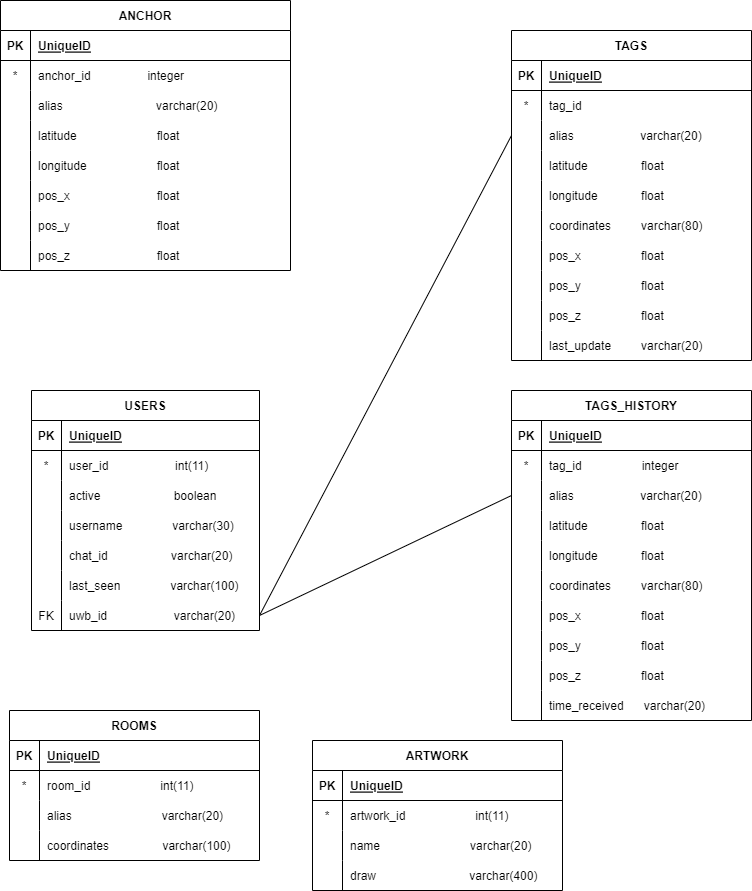
\includegraphics[width=10cm,height=10cm,keepaspectratio]{img/DB COLOSSEUM.drawio.png}
    \caption{Diagrama base de datos.}
    \label{fig:diagram_db}
\end{figure}
\FloatBarrier

\section{Diseño procedimental}
En esta sección se explicará los diagramas de secuencia de una entrada normal a la aplicación web, con todos los sistemas previamente configurados y funcionando.
Para un usuario normal:

\FloatBarrier
\begin{figure}[h]
    \centering
    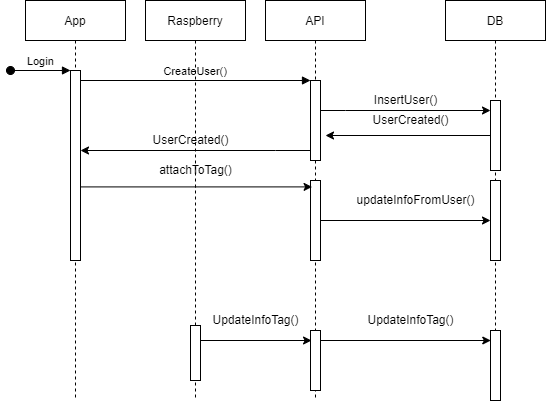
\includegraphics[width=10cm,height=10cm,keepaspectratio]{img/Diagrama procedimental Usuario.drawio (1).png}
    \caption{Diagrama de secuencia de un usuario normal.}
    \label{fig:diagram_seceunce_user}
\end{figure}
\FloatBarrier
Se pueden observar distintas ramas que van hacia la API:
\begin{itemize}
    \item La creación de un usuario en el \textit{login}.
    \item El enlace de un \textit{Tag} a un usuario.
    \item La actualización de la información de posicionamiento desde la \textit{Raspberry}.
\end{itemize}

Se pueden observar que todas las ramas principales utilizan la base de datos.



Para un usuario guía: 
\FloatBarrier
\begin{figure}[h]
    \centering
    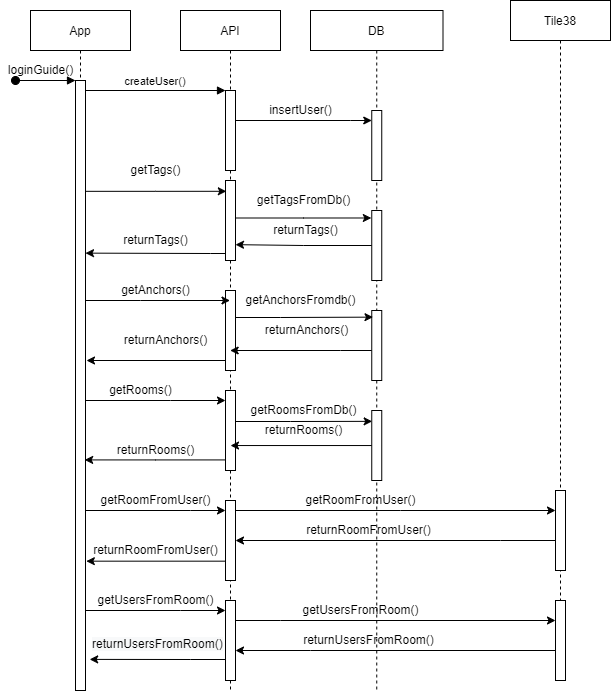
\includegraphics[width=10cm,height=10cm,keepaspectratio]{img/Guide Diagram secuencia.drawio.png}
    \caption{Diagrama de secuencia de un usuario normal.}
    \label{fig:diagram_seceunce_guide}
\end{figure}
\FloatBarrier

Se pueden observar las distintas ramas principales:
\begin{itemize}
    \item La creación de un usuario en el \textit{login}.
    \item La obtención de las \textit{Tags} para mostrarlas en el mapa.
    \item La obtención de los \textit{Anchors} para mostrarlos en el mapa.
    \item La obtención de las \textit{Rooms} para mostrarlas en el mapa.
    \item Cálculo de cuantos usuarios hay en una \textit{Room}.
    \item En que \textit{Room} se encuentra un usuario.
\end{itemize}

Se puede observar que las ultimas dos ramas no hacen uso de la base de datos, sino que calculan el \textit{geofencing} a través del sistema \textit{Tile38} con la información en caché.

\section{Diseño arquitectónico}

\subsection{Modelo-Vista-Controlador (MVC)}

Como ya se ha explicado en partes de la memoria, el uso de \textit{MCV} implica en repartir responsabilidades en 3 partes para intentar mejorar el mantenimiento del código en el futuro y tener un mejor control sobre que hace cada componente.

Este modelo de arquitectura se utiliza en la \textit{API} y la web, a modo que el modelo y el controlador, estarían en la \textit{API}, teniendo el modelo de las bases de datos y la lógica que interactúa con el \textit{ORM} y las peticiones, asimismo la web sería la parte Vista, ya que en la mayoría de peticiones que se hacen son para mostrar información a usuario.
\FloatBarrier
\begin{figure}[h]
    \centering
    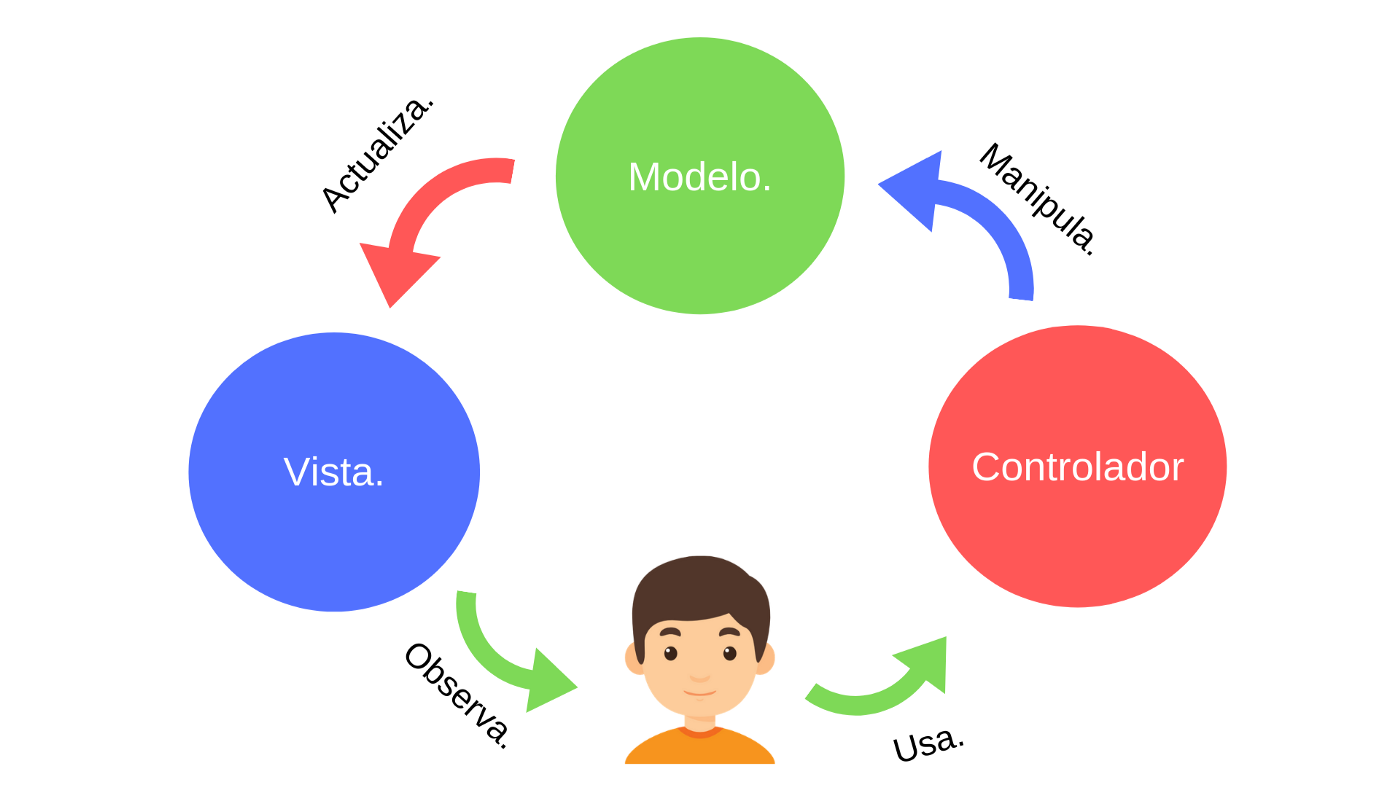
\includegraphics[width=10cm,height=10cm,keepaspectratio]{img/mvc.png}
    \caption{Imagen de flujo en MVC \cite{mvcImag}.}
    \label{fig:mv}
\end{figure}
\FloatBarrier

\subsection{Maestro-Esclavo}

Esta arquitectura se basa en un elemento maestro controla y se comunica con los esclavos, que hacen lo que le pida el maestro.

Esta arquitectura se utiliza en las \textit{Raspberries}, pero como el proyecto no es de gran escala, solo se utilizan componentes maestros.

\FloatBarrier
\begin{figure}[h]
    \centering
    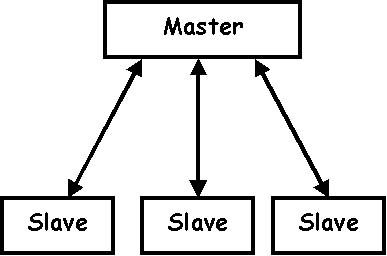
\includegraphics[width=7cm,height=7cm,keepaspectratio]{img/masterslave.jpg}
    \caption{Diagrama de maestro esclavo \cite{masterslaveimg}.}
    \label{fig:diagram_seceunce_guide}
\end{figure}
\FloatBarrier
\subsection{Arquitectura general}
En este apartado se describirá mediante un esquema, la arquitectura general del sistema enseñado el uso de la arquitectura modelo controlador y el uso del \textit{ORM SqlAlchemy} para la conexión con la base de datos.
\FloatBarrier
\begin{figure}[h]
    \centering
    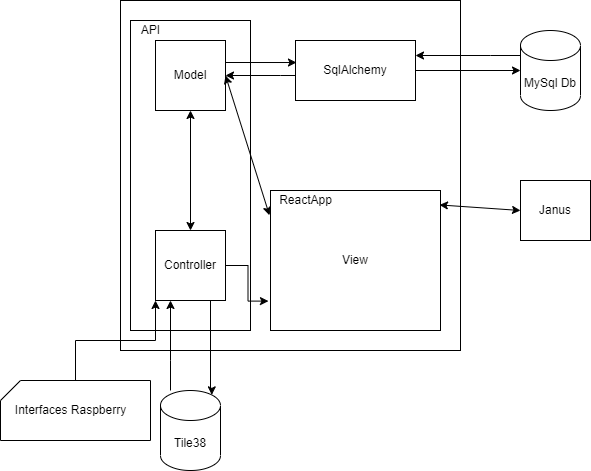
\includegraphics[width=10cm,height=10cm,keepaspectratio]{img/Esquema general del proyecto.drawio (1).png}
    \caption{Diagrama de la arquitectura general.}
    \label{fig:diagram_seceunce_guide}
\end{figure}
\FloatBarrier
\subsection{Diseño de paquetes}
En este subapartado se van a explicar la gestión de paquetes de la aplicación. La estructura general del proyecto es:
\FloatBarrier
\begin{figure}[h]
    \centering
    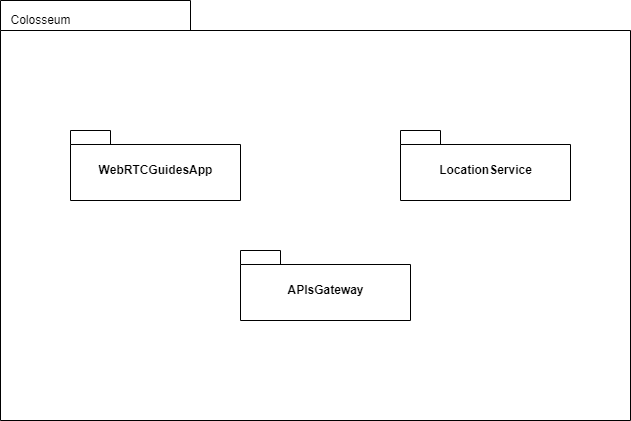
\includegraphics[width=10cm,height=10cm,keepaspectratio]{img/packetsGeneral.drawio (1).png}
    \caption{Paquetes de la aplicación.}
    \label{fig:diagram_seceunce_guide}
\end{figure}
\FloatBarrier
La descripción de cada uno de los paquetes es:
\begin{itemize}
    \item \textit{\textbf{WebRTCGuidesApp}}: Todo el código relacionado con la \textit{webapp} de \textit{React}.
    \item \textit{\textbf{APIsGateway}}: Todo el código relacionado con servicios de la \textit{API}, la base de datos, el servidor web de producción y \textit{Janus}.
    \item \textit{\textbf{LocationService}}: Todo el código relacionado con el servicio de la localización.
\end{itemize}
\FloatBarrier
\begin{figure}[h]
    \centering
    \includegraphics[width=12cm,height=12cm,keepaspectratio]{img/Diseño General depaquetes.drawio.png}
    \caption{Subpaquetes de la aplicación.}
    \label{fig:diagram_seceunce_guide}
\end{figure}
\FloatBarrier

\subsection{Diseño de componentes}
En este apartado se describe como los componentes de la \textit{webapp} interaccionan entre sí:
\FloatBarrier
\begin{figure}[h]
    \centering
    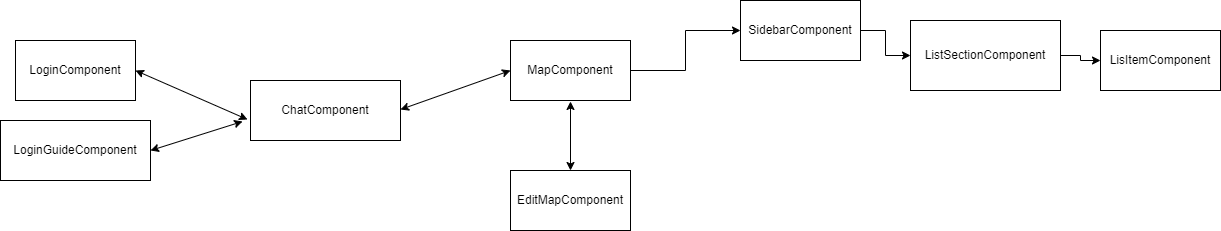
\includegraphics[width=12cm,height=12cm,keepaspectratio]{img/Diagrama de clases Colosseum.drawio.png}
    \caption{Diagrama de componentes de la \textit{webapp}: Interacción.}
    \label{fig:diagram_seceunce_guide}
\end{figure}
\FloatBarrier
\section{Diseño de interfaces}
Para el diseño de las páginas de la \textit{webapp}, se utilizó la herramienta \textit{Figma} para hacer unos bocetos iniciales de las paginas, pero se abandonó el proceso de diseño por falta de tiempo y se intentó adaptar a los diseños ya implementados de la página.

La aplicación web tiene 5 páginas bien diferenciadas siendo estas:
\begin{itemize}
    \item \textit{\textbf{Login}}
    \item \textit{\textbf{LoginGuide}}
    \item \textit{\textbf{Chat}}
    \item \textit{\textbf{Map}}
    \item \textit{\textbf{EditMap}}
\end{itemize}

Algunas imágenes de las interfaces de usuario son son:
\FloatBarrier
\begin{figure}[h]
    \centering
    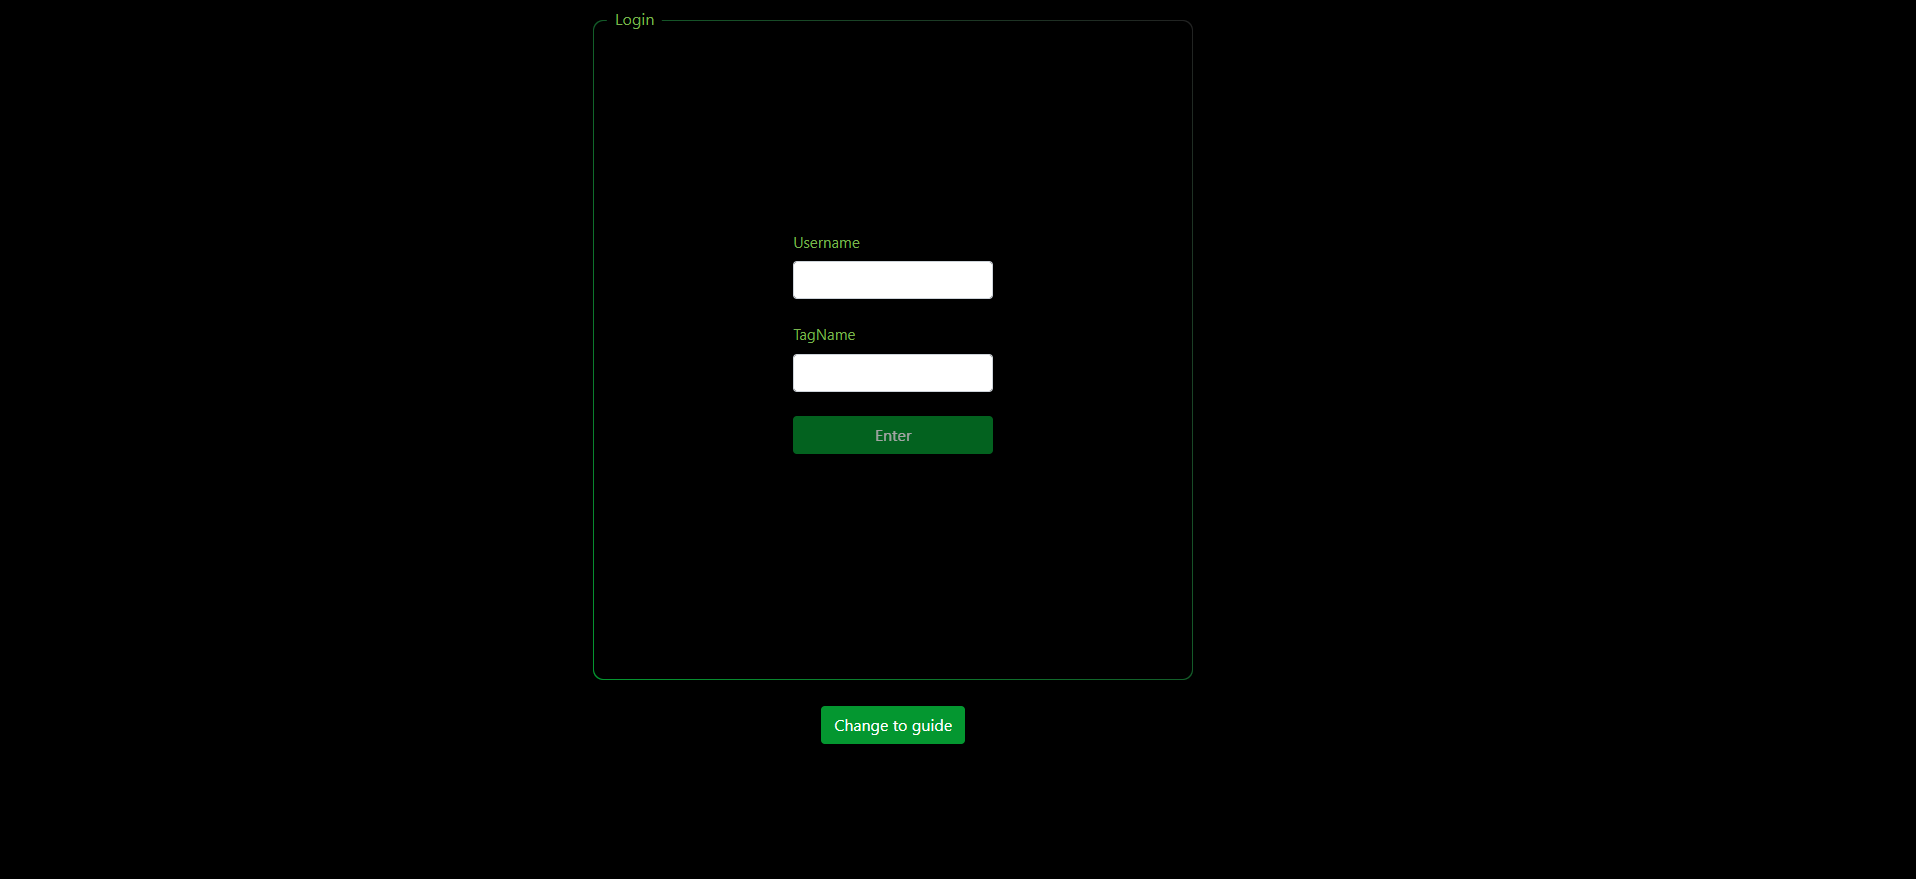
\includegraphics[width=12cm,height=12cm,keepaspectratio]{img/Login.png}
    \caption{Login del usuario.}
    \label{fig:Login del usuario}
\end{figure}
\FloatBarrier
\FloatBarrier
\begin{figure}[h]
    \centering
    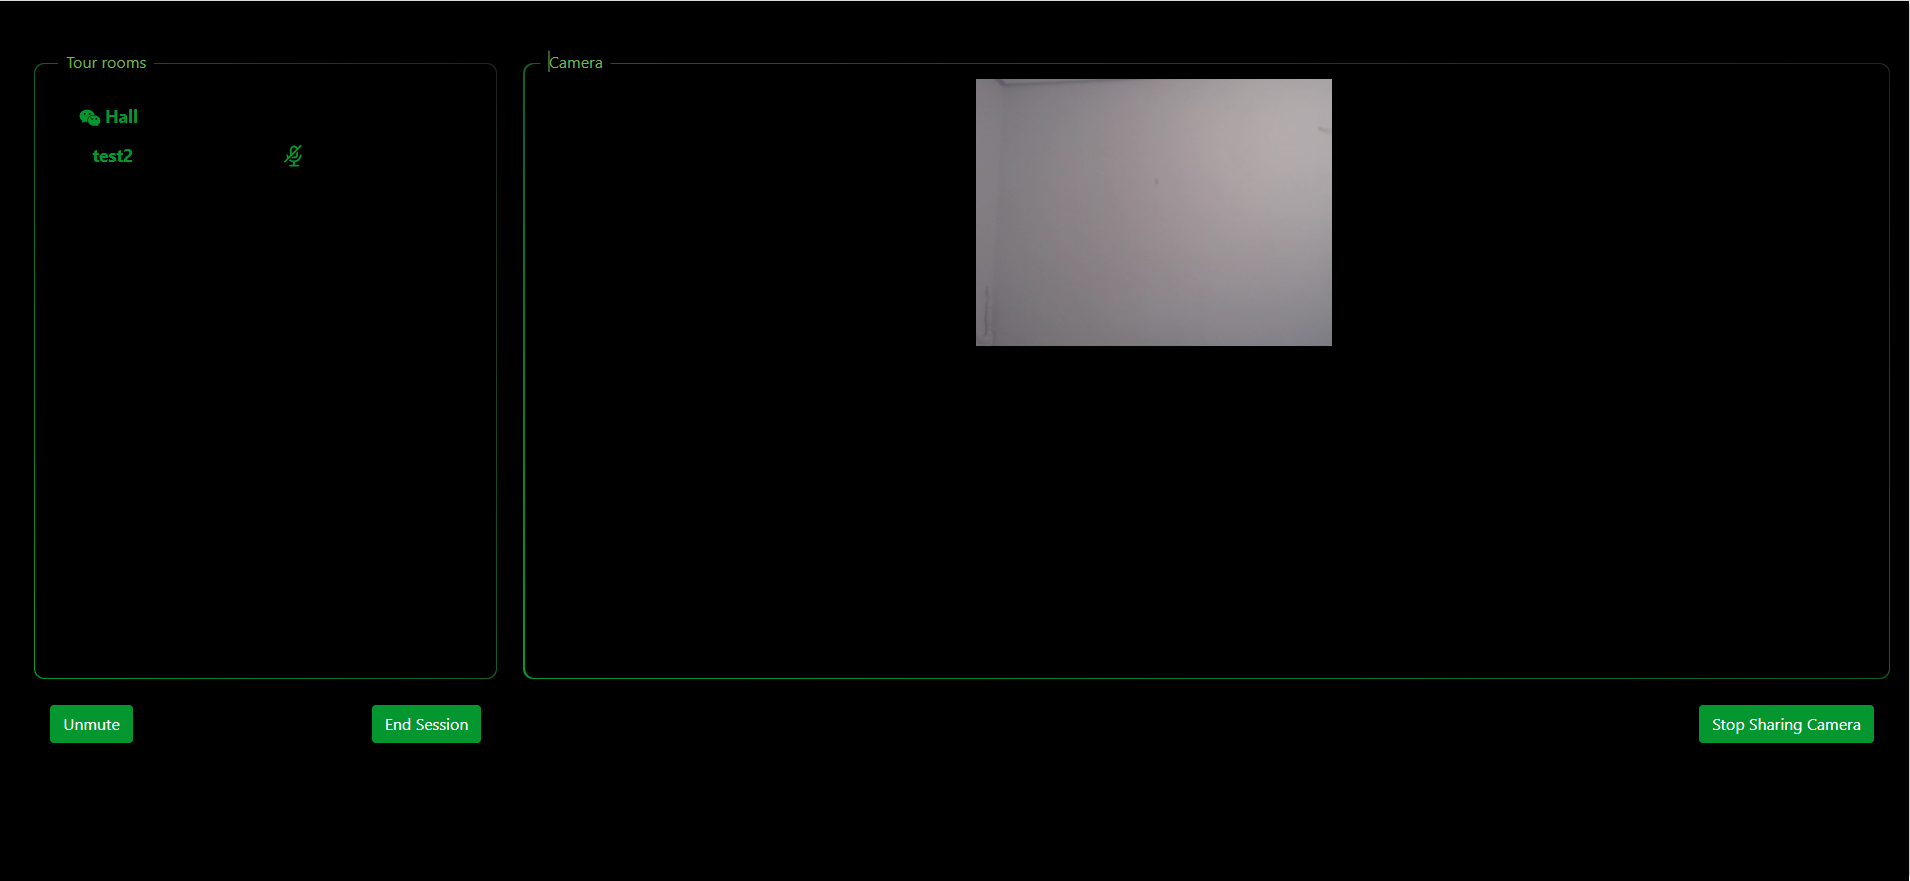
\includegraphics[width=12cm,height=12cm,keepaspectratio]{img/UserChatDesktop.png}
    \caption{Chat desde la vista del usuario.}
    \label{fig:Chat desde la vista del usuario}
\end{figure}
\FloatBarrier
\FloatBarrier
\begin{figure}[h]
    \centering
    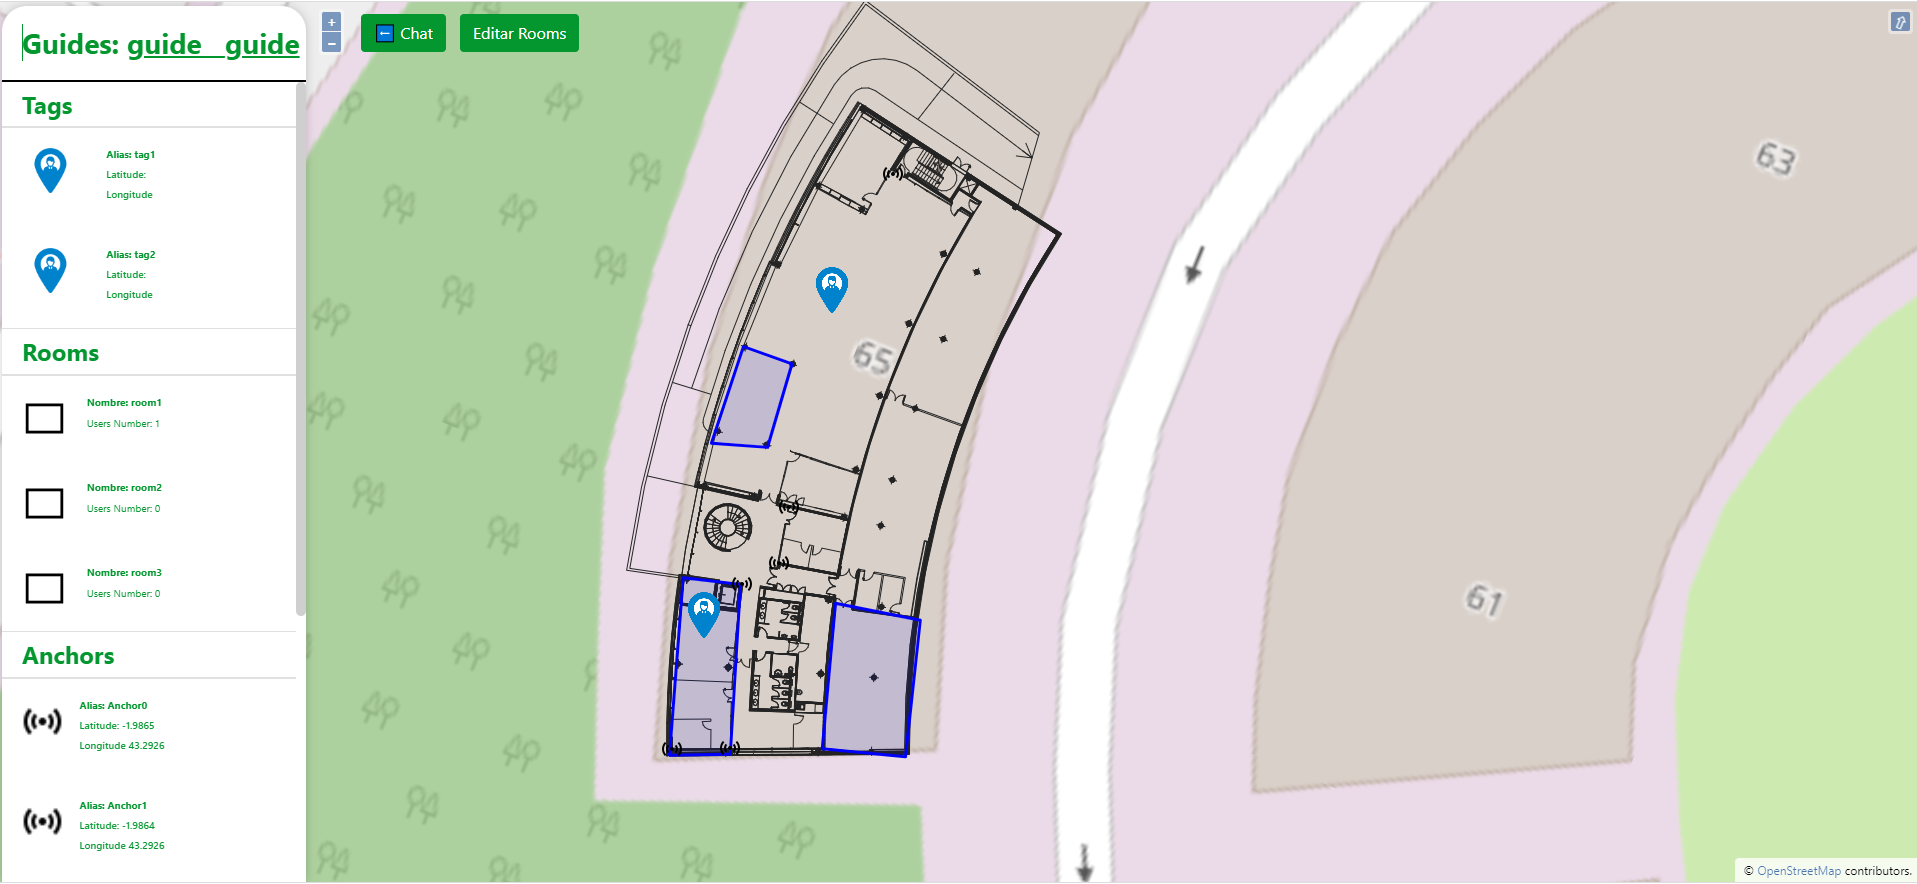
\includegraphics[width=12cm,height=12cm,keepaspectratio]{img/Map.png}
    \caption{Mapa del guía.}
    \label{fig:Mapa del guía}
\end{figure}
\FloatBarrier

Por otro lado el siguiente diagrama muestra el flujo de navegabilidad por las paginas de los usuarios:

\FloatBarrier
\begin{figure}[h]
    \centering
    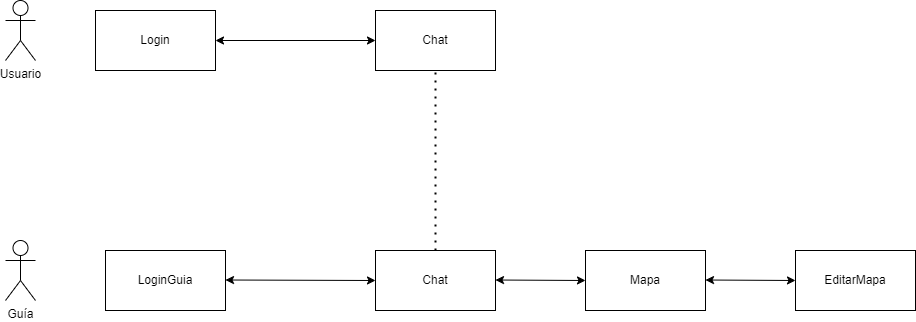
\includegraphics[width=12cm,height=12cm,keepaspectratio]{img/Flujo de navegabilidad.png}
    \caption{Diagrama de flujo de navegabilidad de los usuarios por las páginas.}
    \label{fig:Flujo de navegabilidad de los usuarios por las páginas}
\end{figure}
\FloatBarrier
\apendice{Documentación técnica de programación}
\section{Introducción}
En este apéndice se va a describir la documentación técnica de programación, incluyendo la estructura de directorios, manual para el programador, despliegue de herramientas para desarrollo, ejecución del proyecto y pruebas del sistema.

\section{Estructura de directorios}
El proyecto tiene una estructura de directorio tal que:
\begin{itemize}
    \item \textit{./doc/}: Todos los archivos relacionados con la documentación del proyecto.
    \item \textit{./WebRTCGuidesApp/}: Todos los archivos relacionados con la \textit{webapp}.
    \item \textit{./WebRTCGuidesApp/src/}: Todos los archivos relacionados con los componentes de \textit{React}.
    \item \textit{./APIsGateways/openapi-server-container/openapi\_server/}: Todos los archivos relacionados con la \textit{API}.
    \item \textit{./APIsGateways/openapi-server-container/openapi\_server/config/}: Todos los archivos relacionados con la configuración de la API.
    \item \textit{./APIsGateways/openapi-server-container/openapi\_server/controllers/}: Todos los archivos relacionados con los controladores.
    \item \textit{./APIsGateways/openapi-server-container/openapi\_server/models/}: Todos los archivos relacionados con los modelos y esquemas del ORM.
    \item \textit{./APIsGateways/openapi-server-container/openapi\_server/openapi/}: El archivo de extensión \textit{.yaml} que tiene las especificaciones de la \textit{API}.
    \item \textit{./APIsGateways/}: Todos los servicios que funcionan en el mismo \textit{docker-compose}.

\end{itemize}

\section{Manual del programador}
En este apartado se van a explicar los puntos necesarios para que se pueda entender el despliegue de la aplicación para desarrollar sobre ella.

Durante este proyecto se ha trabajado con \textit{Github}, por lo que el repositorio del proyecto está allí, para obtenerlo primero tendríamos que clonar el repositorio:

\subsection{Clonar repositorio}

Antes de nada es necesario tener instalado \textit{Git} en la consola de comandos, ya bien sea en \textit{Windows} o en \textit{Linux} (a veces viene de serie):

\begin{itemize}
    \item 1. Abrir el \textit{bash} de \textit{git}, donde nos interese clonar el repositorio.
    \item 2. Escribir el comando: 
    \item 3. Una vez tenemos el repositorio, podremos acceder y tendremos que cambiar a la rama de \textit{dev} con el comando: \textit{git checkout dev}.
\end{itemize}
\FloatBarrier
\begin{figure}[h]
    \centering
    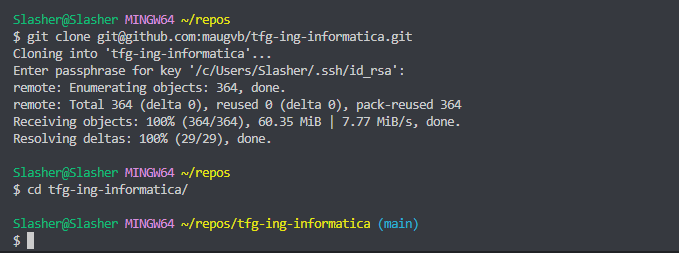
\includegraphics[width=12cm,height=12cm,keepaspectratio]{img/git.png}
    \caption{Clonado de repositorio de la herramienta \textit{Github} desde \textit{WSL 2}.}
    \label{fig:Flujo de navegabilidad de los usuarios por las páginas}
\end{figure}
\FloatBarrier

\subsection{Entorno de desarrollo}
Para el entorno de desarrollo se ha utilizado\textit{\textbf{Visual Studio Code}}.
\begin{itemize}
    \item 1. Si no lo tuviésemos descargado, lo descargaríamos.
    \item 2. Teniendo \textit{WSL 2} en \textit{Windows}, o ejecutando en \textit{Ubuntu}, desde la línea de comandos nos aseguramos que tenemos el comando code instalado.
    \item 3. Desde la consola de comando vamos a la carpeta del proyecto.
    \item 4. Escribimos el siguiente comando: \textit{"code ."}, que abrirá la carpeta del proyecto directamente en la ventana de \textit{Visual Studio Code}.

\end{itemize}
\section{Compilación, instalación y ejecución del proyecto}
En este apartado se explicará el despliegue de la aplicación.
\subsection{Compilación}
En este subapartado nos centraremos en la compilación de nuestro proyecto.
\begin{itemize}
    \item \textit{\textbf{Webapp}}: para la compilación del proyecto en modo desarrollador, tendríamos que ir a la carpeta \textit{/WebRTCGuidesApp} y ejecutar el comando \textit{yarn dev}, previamente deberemos de haber lanzado el comando \textit{yarn install} para la instalación de los \textit{node\_modules}, que son las dependencias externas de la aplicación. Después de lanzar el comando \textit{yarn dev} nuestra aplicación compilada estará corriendo en \textit{https://localhost:3000}.
    \item \textit{\textbf{API}}: No es un proceso de compilación, pero si hacemos algún cambio en el código de la \textit{API}, para que se actualicen os cambios en el contenedor, debemos ir a la carpeta \textit{APIsGateway} y lanzar el comando \textit{docker-compose build}.
\end{itemize}
\subsection{Ejecución}
Para la ejecución de los servicios, tenemos un \textit{Makefile} en la raíz del proyecto donde:
\begin{itemize}
    \item Para hacer deploy de la app debemos ejecutar el comando \textit{make run-build}.
    \begin{itemize}
        \item \textit{API} en \textit{http://ip-local:8080}
        \item Web en \textit{https://ip-local:80}
    \end{itemize}
    \item Iniciar servicios en modo \textit{developer} tendremos que ejecutar el comando \textit{make dev}. Donde quedarán activos los servicios:
    \begin{itemize}
        \item \textit{API} en \textit{http://localhost:8080}
    \end{itemize}
    
    \item Para eliminar la base de datos debemos de ejecutar el comando \textit{make clean}.
\end{itemize}
\subsection{Despliegue Hardware en entorno físico}
Para el despliegue en un entrono real debemos:
\begin{itemize}
    \item Cambiar \textit{firmware} de las placas en función de los roles: \textit{Anchors}, \textit{Tags} y \textit{Listeners}.
    \item Colocar los \textit{Anchors} y el \textit{Listener}, y colocarlos en las salas.
    \item Con las coordenadas de los \textit{Anchors} en el mapa y una \textit{Room} dibujada, modificamos el código en la \textit{raspberry} para hacer la traslación. 
    \item Y ya obtendríamos información en la \textit{webapp} de los \textit{Tags}.
\end{itemize}
\section{Pruebas del sistema}
En este proyecto han habido dos tipos de pruebas:
\begin{itemize}
    \item Pruebas generales. Estas pruebas se realizaron a modo de auditorías para comprobar los progresos en la aplicación, pasando en todos los estándares de la empresa.
    \item Prueba de estrés. Prueba en la que se lleva al límite una parte de la aplicación para ver su respuesta.
\end{itemize}
\subsection{Prueba 1}
    En esta prueba se utilizaron una sala especifica de la oficina, donde se colgaron cuadros, con una red de reconocimiento de cuadros, ya entrenada. Además se comprobó la fiabilidad de la localización \textit{indoor} con 3 \textit{Anchors} y 1 \textit{Tag} a modo de usuario.
    
    El usuario lleva una \textit{tablet} con la web funcionando, compartiendo vídeo y audio, y apunta con la cámara a una de las obras de arte, así el guia puede dibujar sobre ella.
\subsection{Prueba 2}
    En esta prueba se utilizaron dos salas especificas de la oficina, donde se colgaron cuadros, con una red de reconocimiento de cuadros, ya entrenada. Además se comprobó la fiabilidad de la localización indoor con 3 \textit{Anchors} por sala y 1 \textit{Tag} a modo de usuario.
    
    El usuario lleva una \textit{tablet} con la web funcionando, compartiendo vídeo y audio, y apunta con la cámara a una de las obras de arte, así el guia puede dibujar sobre ella.
\subsection{Prueba 3}
    En esta prueba se utilizaron una sala especifica de la oficina, donde se colgaron cuadros, con una red de reconocimiento de cuadros, ya entrenada. Además se comprobó la fiabilidad de la localización indoor con 3 \textit{Anchors} y 2 \textit{Tag} a modo de usuario.
    
    Los usuarios llevan una \textit{tablet} con la web funcionando, compartiendo vídeo y audio, y apuntan con la cámara a una de las obras de arte, así el guia puede dibujar sobre ella.

\subsection{Prueba de estrés}
La página de mapa, la \textit{API} y la base de datos, se someten a una prueba de estrés con el \textit{script} en la carpeta \textit{WebRTCGuidesAPP/test/TagsInMap.py}. Cuando se ejecuta añade un \textit{Tag} y un usuario con nombres aleatorios enlazados. Las \textit{Tags} se generan con coordenadas aleatorias dentro de un rango determinado, para poder comprobar el comportamiento del mapa en tiempo real.
\apendice{Documentación de usuario}

\section{Introducción}
En este punto de procederá a explicar el manual del usuario para el uso de la aplicación. Las indicaciones se hacen sobre un sistema \textit{Windows}, pero al ser una aplicación web, con tener instalado el buscador \textit{Chrome} en su última versión, servirá para poder interactuar con el sistema.

\section{Requisitos de usuarios}
Los requisitos para los usuarios son muy simples, al ser una aplicación web, funcionaria en cualquier buscador, pero se recomienda:
\begin{itemize}
    \item Ordenador, tablet o dispositivo móvil con mínimo 2 GB de memoria \textit{RAM}.
    \item Buscador \textit{Chrome} en versión 88.0 o superior.
\end{itemize}
\section{Instalación}
Al ser una aplicación web, no requiere de instalaciones extra para poder funcionar, lo que si es necesario es el despliegue de placas \textit{UWB} y las \textit{Raspberries} necesarias para que el sistema funcione.

\section{Manual del usuario}
\subsection{Usuario}
El usuario tiene diversas funcionalidades. Al entrar se encuentra en la pagina de \textit{Login}.
\FloatBarrier
\begin{figure}[h]
    \centering
    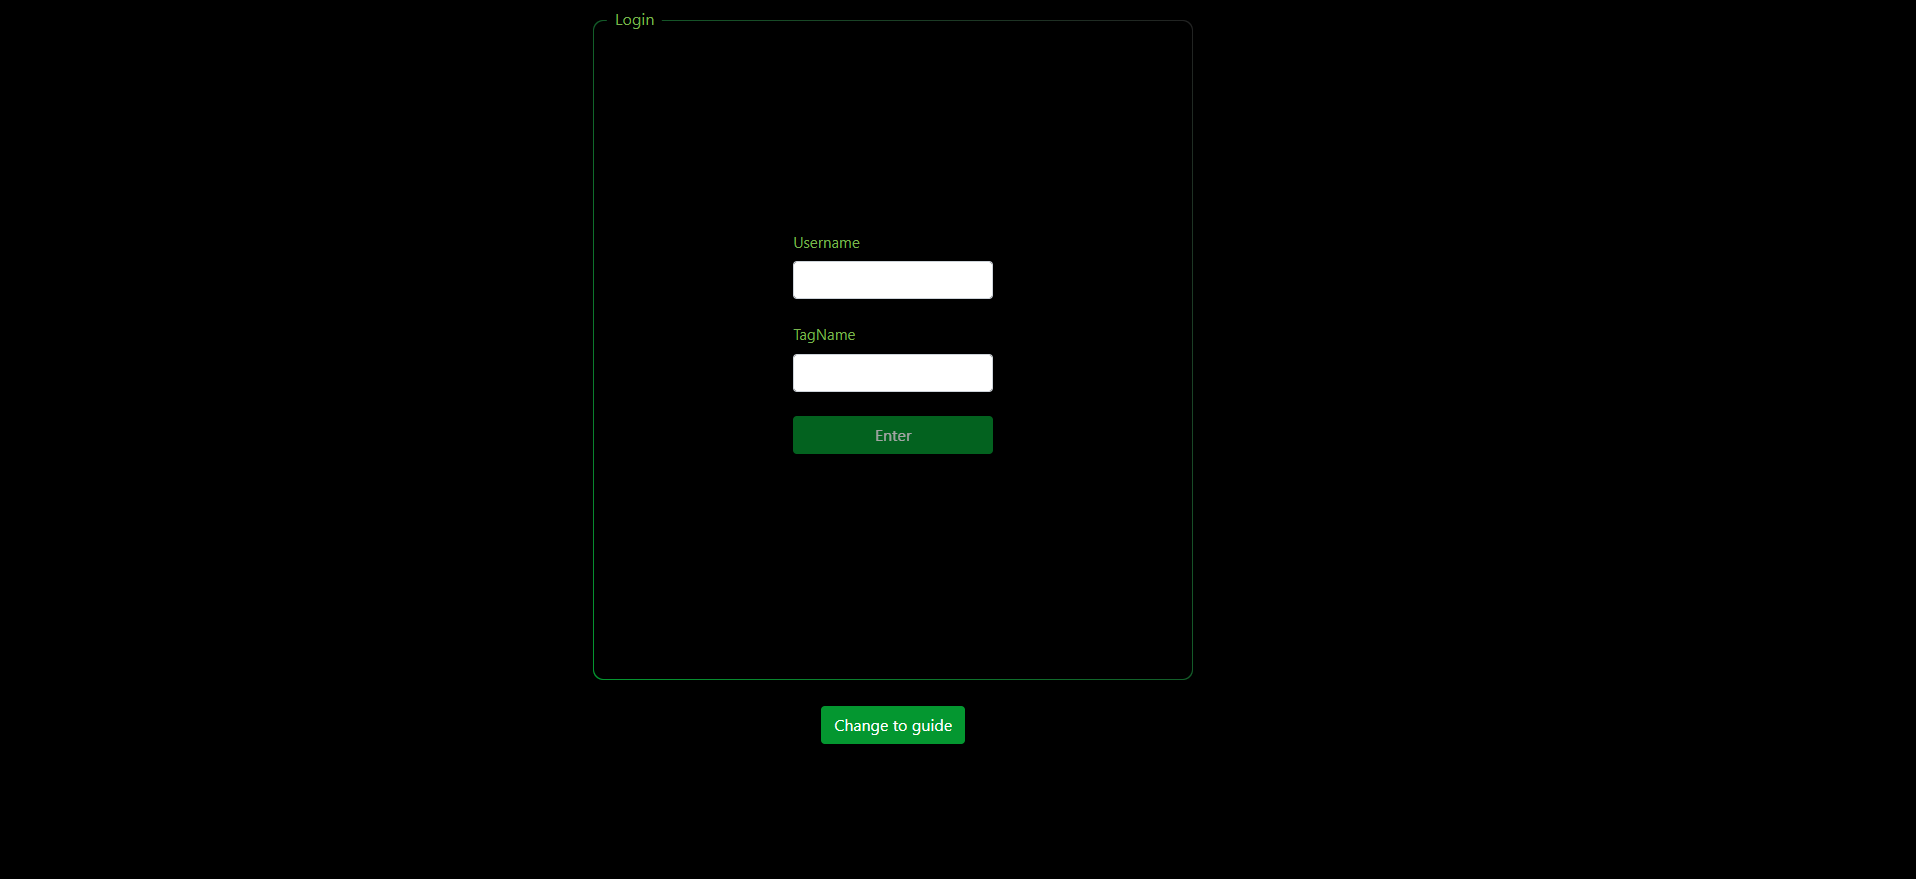
\includegraphics[width=10cm,height=10cm,keepaspectratio]{img/Login.png}
    \caption{Página de \textit{Login en la vista Usuario}.}
    \label{fig:Página de Login en la vista Usuario}
\end{figure}
\FloatBarrier

Una vez hace el \textit{Login} correctamente y se le enlaza con una \textit{Tag} pasa a la página del \textit{chat}, donde se le asigna una visita, y comparte vídeo y audio.


La aplicación tendrá acceso a la cámara y se podrán identificar obras de arte. Pudiendo recibir del guía las indicaciones pintadas sobre una capa \textit{canvas} sobre la obra de arte. Como último paso se podrá hacer logout, quitando en enlace usuario-tag de la base de datos.
\FloatBarrier
\begin{figure}[h]
    \centering
    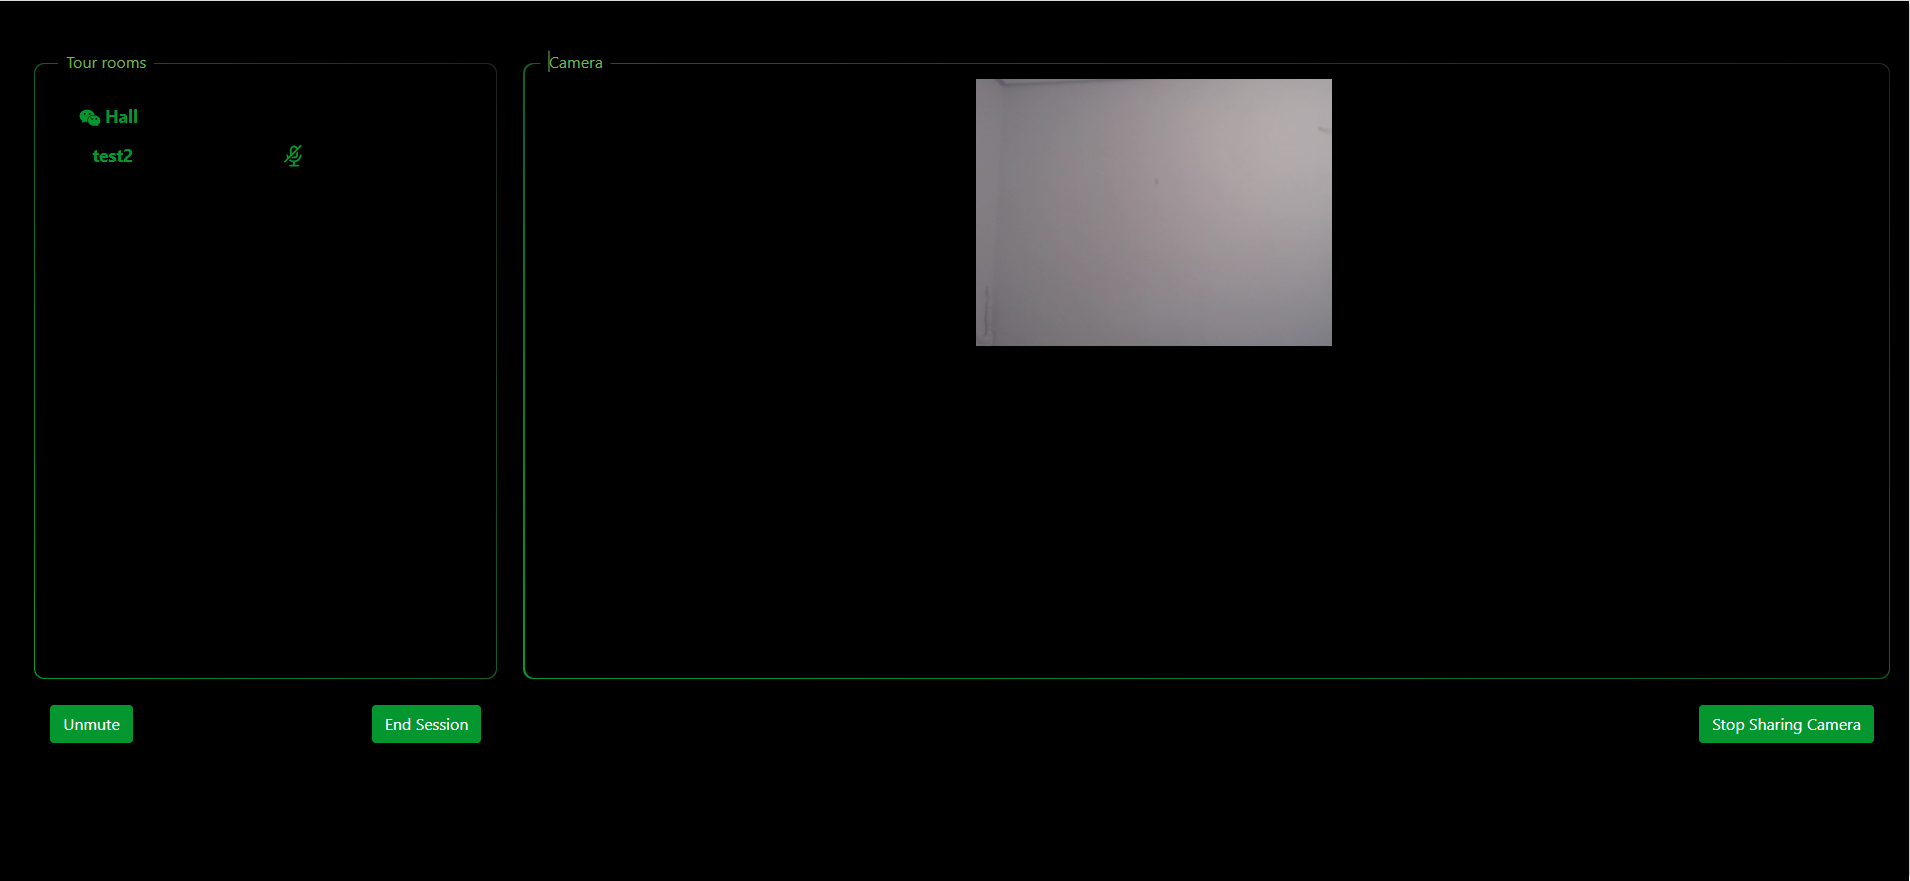
\includegraphics[width=10cm,height=10cm,keepaspectratio]{img/UserChatDesktop.png}
    \caption{Página chat desde la visión de usuario.}
    \label{fig:Página chat desde la visión de usuario}
\end{figure}
\FloatBarrier

Esta pagina de \textit{chat} cuenta con un diseños para ser visualizados desde múltiples dispositivos, diseños \textit{responsives}, ya que están pensados para ser usado por el usuario desde una \textit{tablet} o un dispositivo móvil.
\FloatBarrier
\begin{figure}[h]
    \centering
    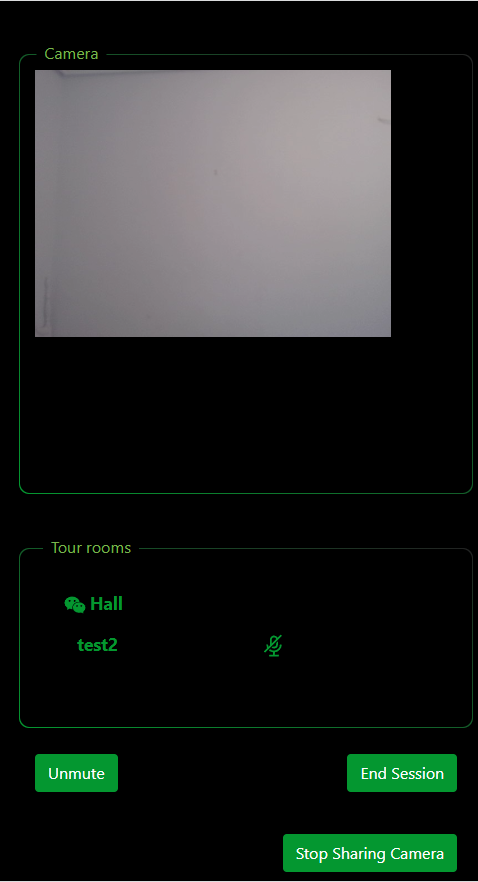
\includegraphics[width=10cm,height=10cm,keepaspectratio]{img/UserChatMobile.png}
    \caption{Página de chat desde la visión de un usuario con un dispositivo móvil.}
    \label{fig:diagram_seceunce_guide}
\end{figure}
\FloatBarrier
\subsection{Guía}

El usuario guia ha de hacer \textit{login} con un nombre especifico, si se hace correctamente se pasará a la sala del \textit{chat}.
\FloatBarrier
\begin{figure}[h]
    \centering
    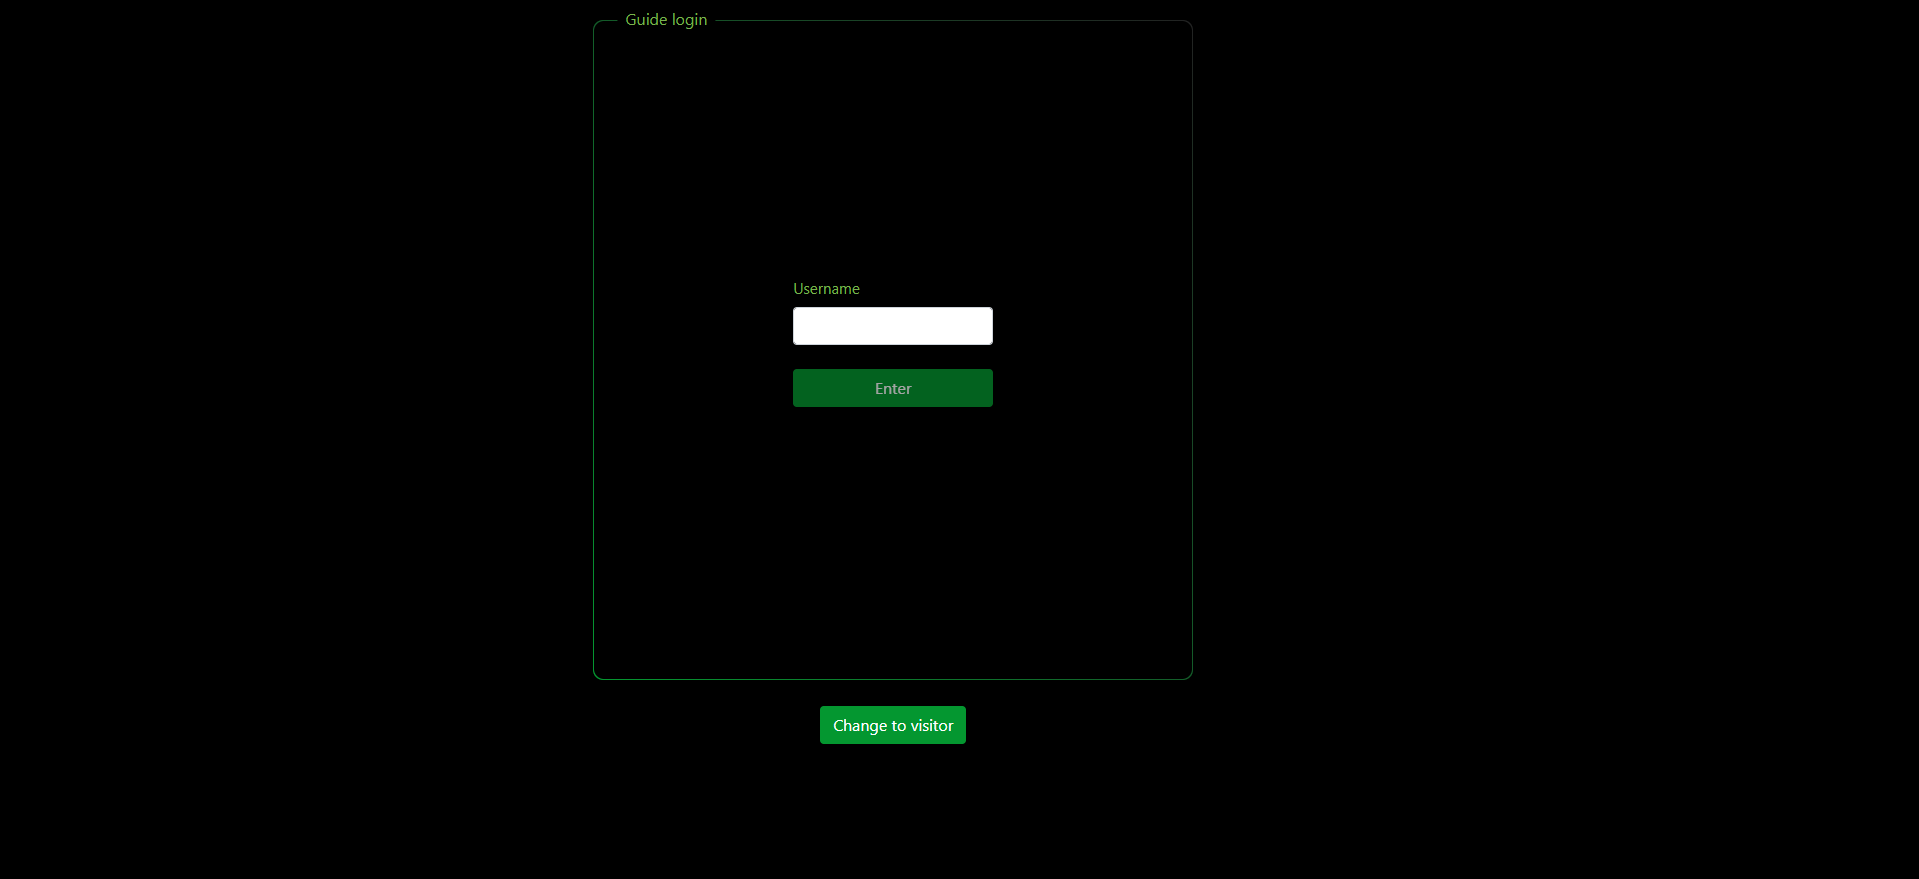
\includegraphics[width=10cm,height=10cm,keepaspectratio]{img/LoginGuide.png}
    \caption{Página \textit{Login} desde la visión del guía.}
    \label{fig:diagram_seceunce_guide}
\end{figure}
\FloatBarrier
En esta sala se tendrá una visión general de los usuarios en las visitas, hay una característica de \textit{drag and drop} que permite meter y sacar usuarios de tours arrastrándolos y soltándolos.


Además se podrán ver las cámaras y audio, teniendo control por separado, de hasta 4 usuarios simultáneamente. Se podrá ir desde un botón a la página de mapa.
\FloatBarrier
\begin{figure}[h]
    \centering
    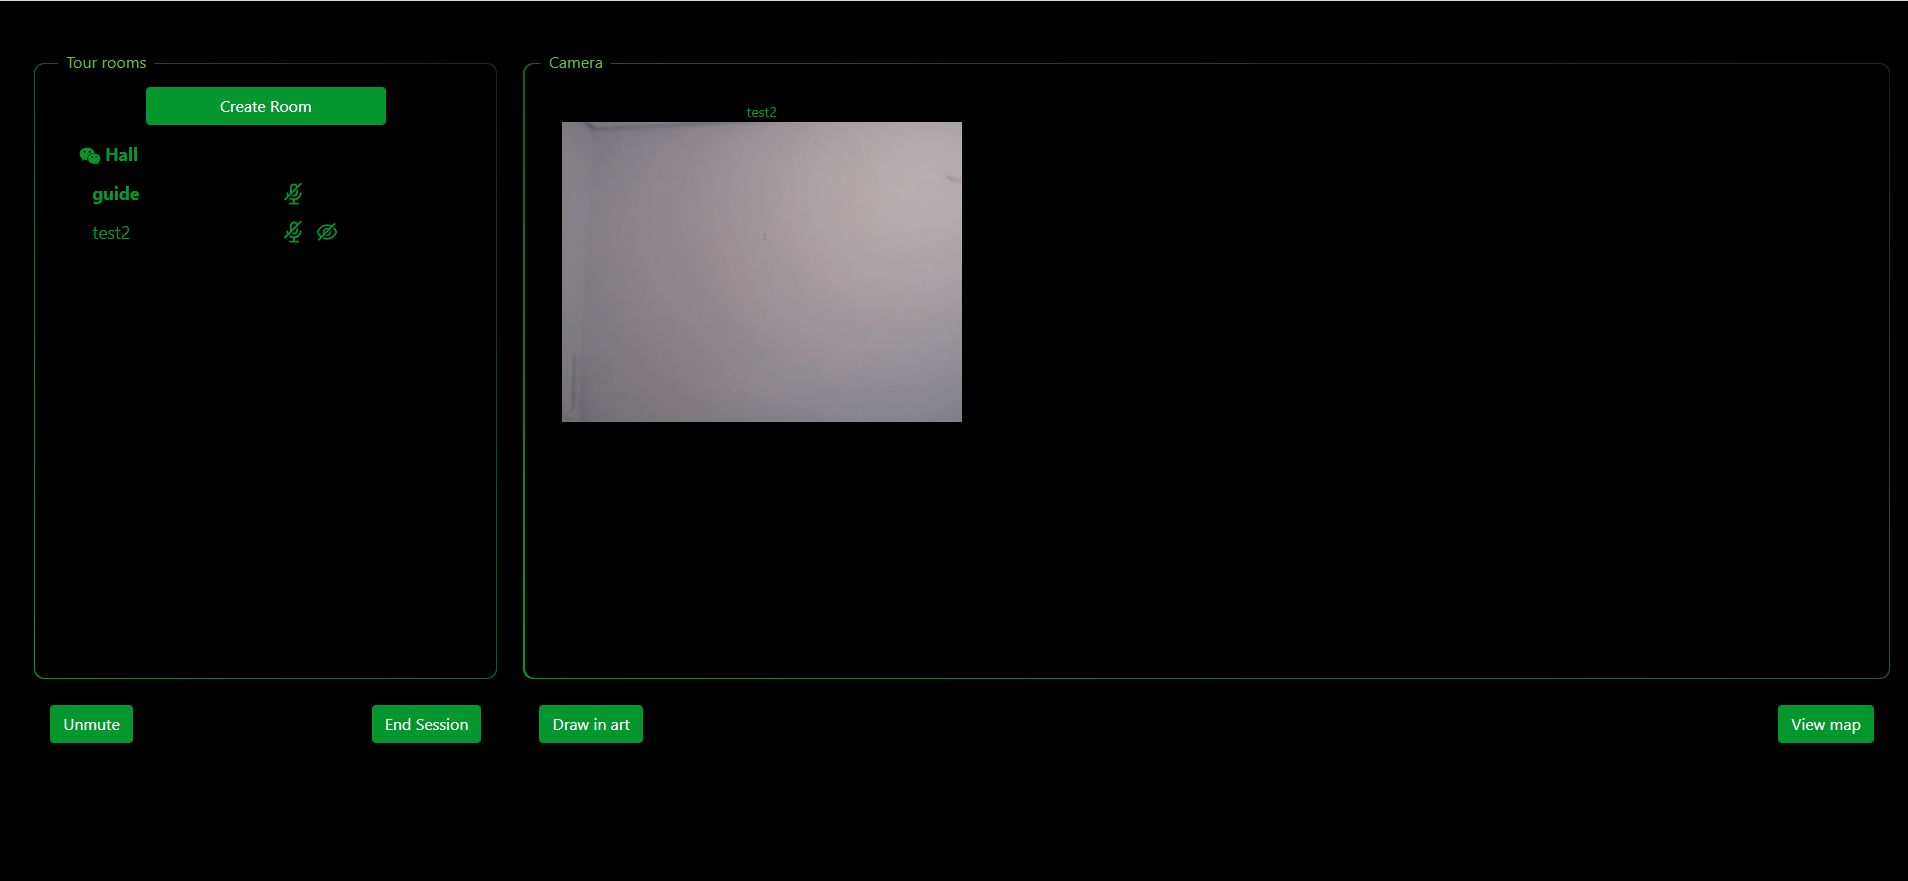
\includegraphics[width=10cm,height=10cm,keepaspectratio]{img/GuideChatDesktop.png}
    \caption{Página \textit{chat} desde la visión del guía.}
    \label{fig:diagram_seceunce_guide}
\end{figure}
\FloatBarrier

En la pagina de mapa, tendremos un \textit{sidebar} con toda la información relevante de los \textit{Anchors}, \textit{Tags} y \textit{Rooms}. De fondo se verá el mapa con \textit{Anchors}, \textit{Tags} y \textit{Rooms} renderizado a tiempo real.

Además se puede pinchar sobre \textit{Anchors} y \textit{Tags}, dando información extra en un segundo \textit{sidebar}.
\FloatBarrier
\begin{figure}[h]
    \centering
    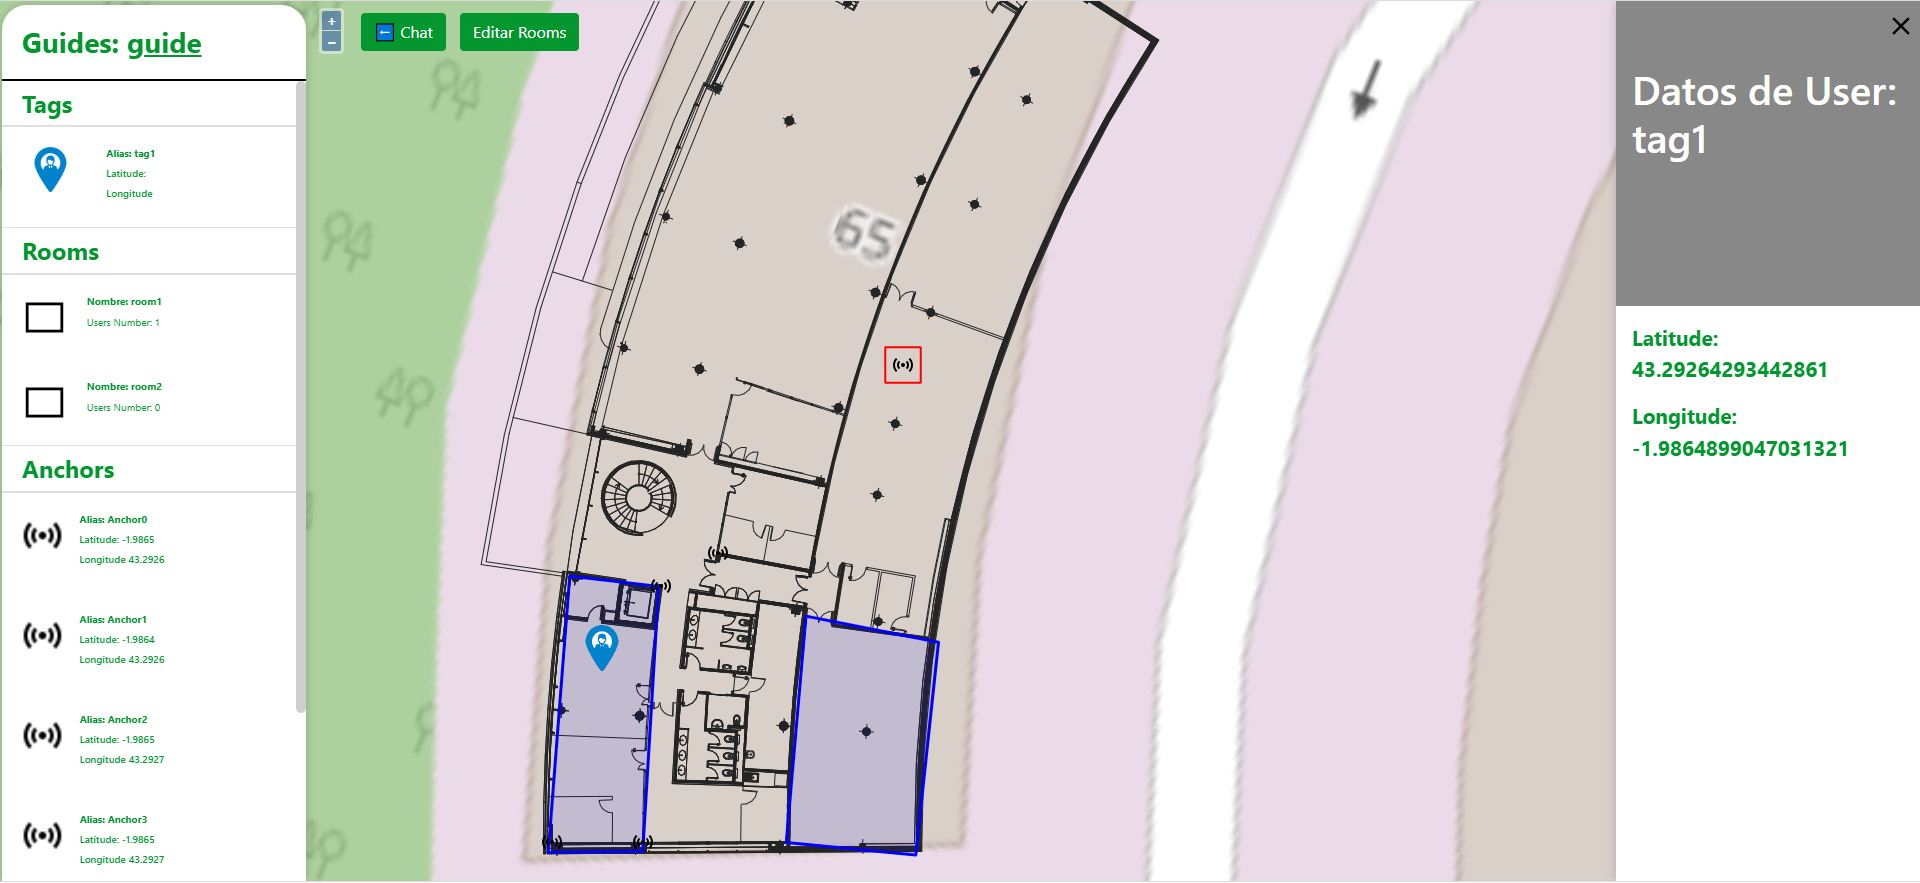
\includegraphics[width=10cm,height=10cm,keepaspectratio]{img/tagsidebar.png}
    \caption{Página Mapa con el \textit{sidebar} de visualización de un único \textit{Tag}.}
    \label{fig:diagram_seceunce_guide}
\end{figure}
\FloatBarrier

Si pinchamos sobre un \textit{Anchor}, en el segundo \textit{sidebar} se podrá permitir el movimiento del \textit{Anchor} arrastrándolo y soltándolo, persistiendo su nueva posición en la base de datos si así lo deseamos mediante el botón "Guardar Anchor" . 
\FloatBarrier
\begin{figure}[h]
    \centering
    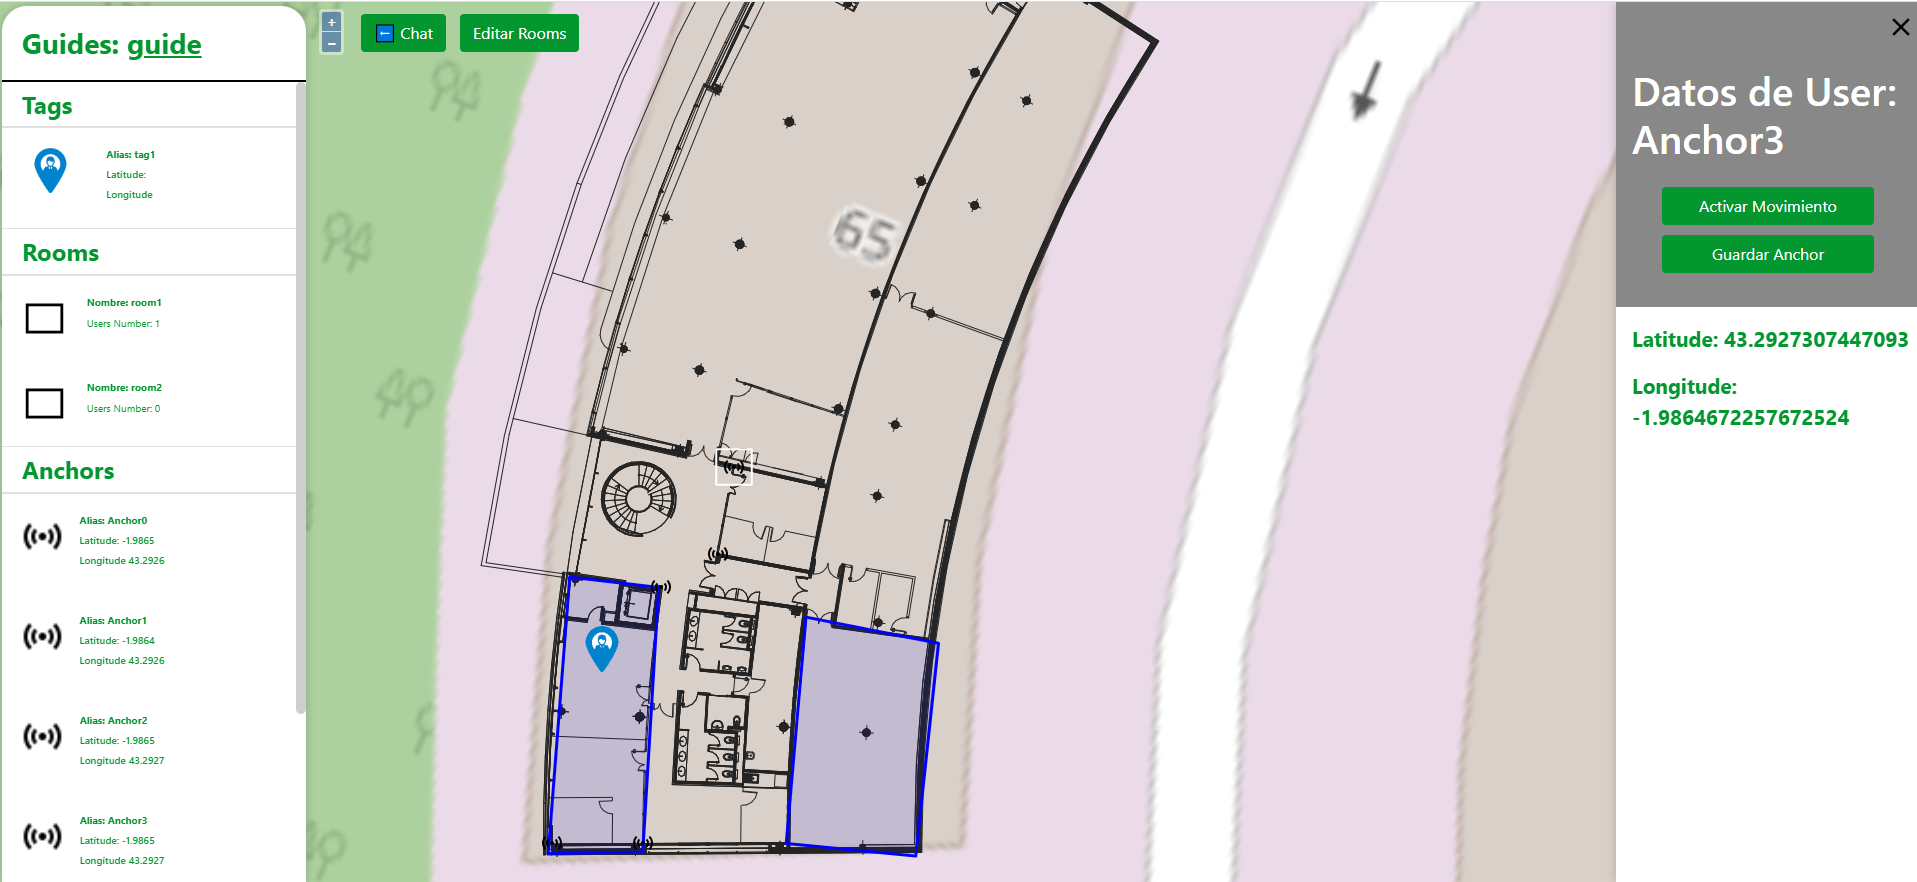
\includegraphics[width=10cm,height=10cm,keepaspectratio]{img/anchorsidebar.png}
    \caption{Página Mapa con el \textit{sidebar} de control de un \textit{Anchor}.}
    \label{fig:Página Mapa con el sidebar de control de un Anchor}
\end{figure}
\FloatBarrier
Si el \textit{Anchor} ha sido movido pero no guardado, saldrá un cuadrado rojo.
\FloatBarrier
\begin{figure}[h]
    \centering
    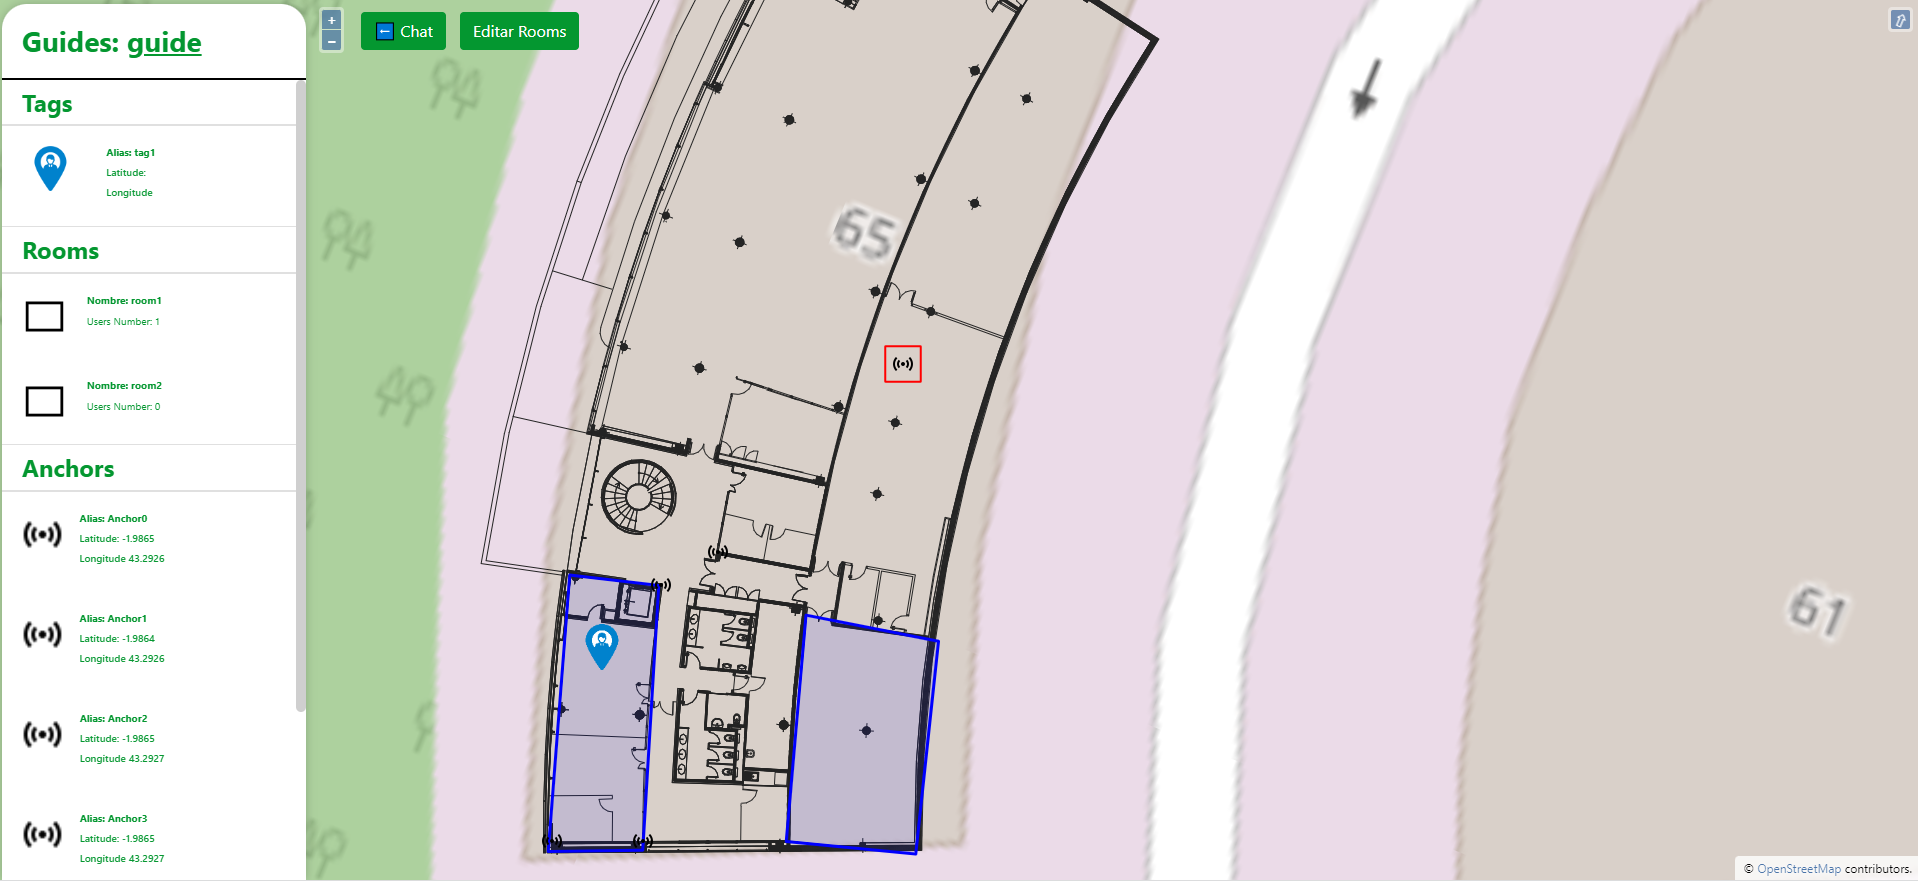
\includegraphics[width=10cm,height=10cm,keepaspectratio]{img/anchorsidebarMoved.png}
    \caption{Página Mapa gestionando la posición de un \textit{Anchor} sin guardar desde la vista del guía.}
    \label{fig:Página Mapa gestionando la posición de un Anchor sin guardar desde la vista del guía}
\end{figure}
\FloatBarrier

Desde la página de Mapa podemos ir a la página de EditarRoom, donde podemos crear y eliminar \textit{Rooms}.



La vista general es el mapa cargado solo con las \textit{Rooms} y un \textit{sidebar} con las \textit{Rooms} existentes y un botón para eliminar. Se podrán dibujar las \textit{Rooms} con el polígono que queramos y guardarlo en la base de datos, mediante el control de botones de la parte superior de la página.

\FloatBarrier
\begin{figure}[h]
    \centering
    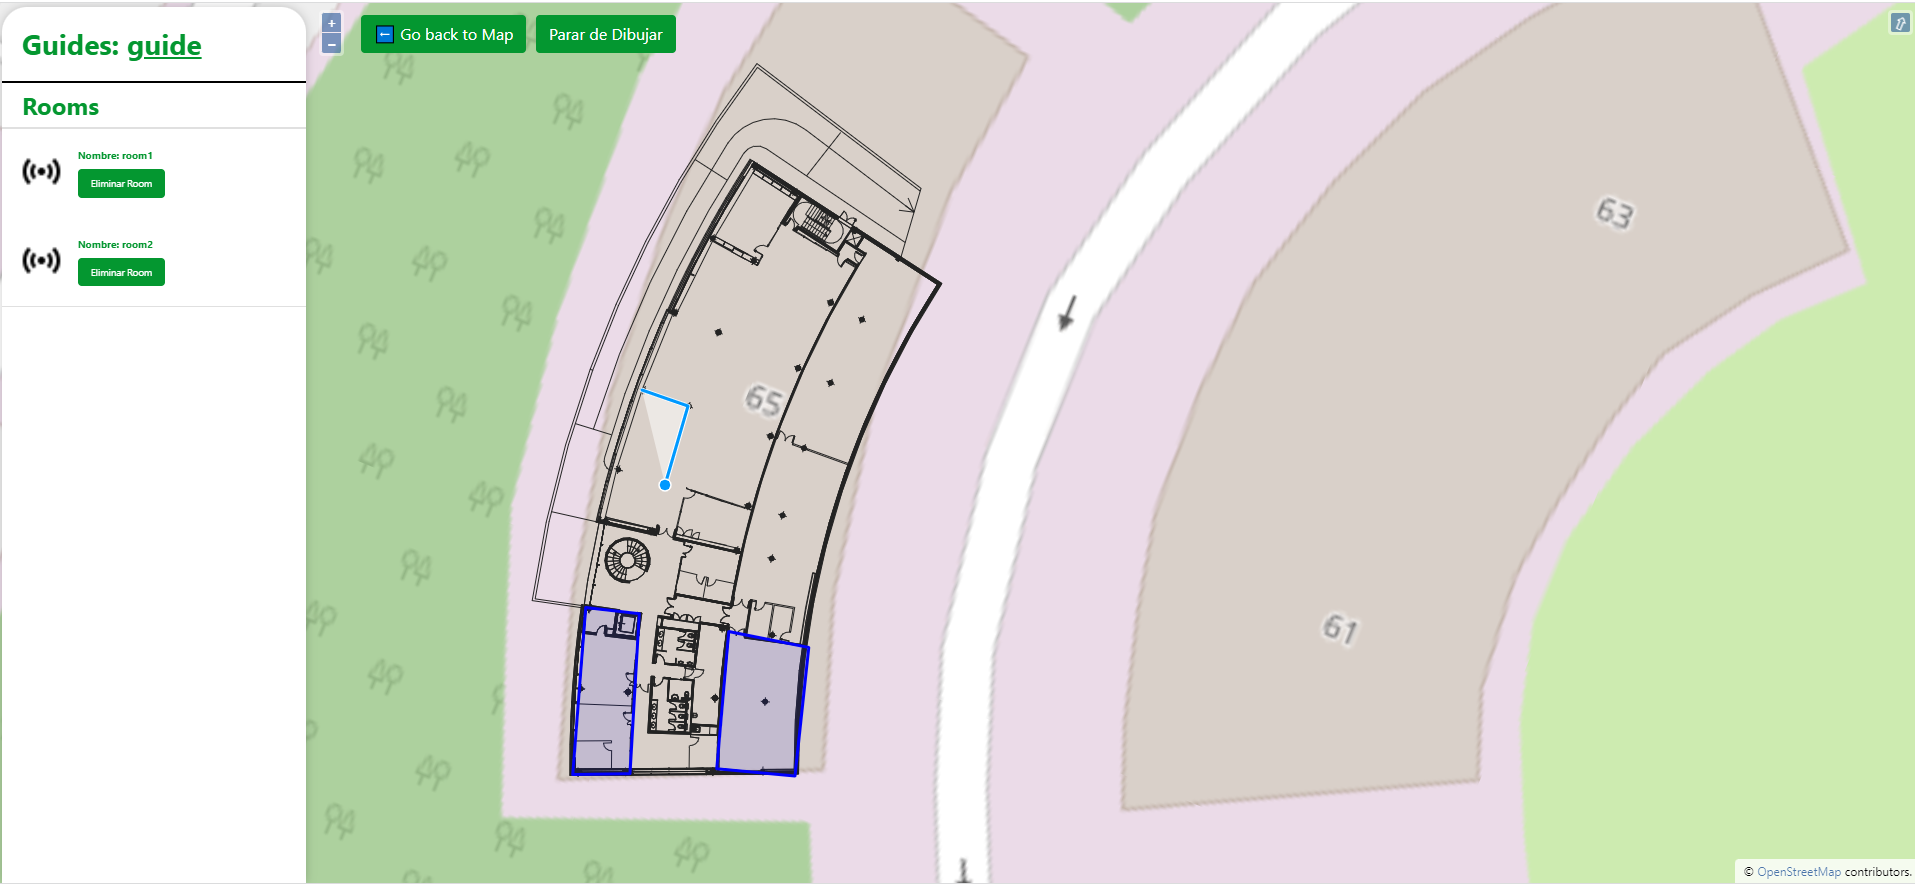
\includegraphics[width=10cm,height=10cm,keepaspectratio]{img/EditRoom.png}
    \caption{Página \textit{EditarRoom} de la vista del guía.}
    \label{fig:Página Editar Room de la vista del guía}
\end{figure}
\FloatBarrier





\bibliographystyle{plain}
\bibliography{bibliografiaAnexos}

\end{document}
